\documentclass[11pt]{article} %
\usepackage{times}
%
\usepackage[letterpaper, left=1in, right=1in, top=1in, bottom=1in]{geometry}

\usepackage[utf8]{inputenc} %
\usepackage[T1]{fontenc}    %

%
%
%
\usepackage{natbib}
%
\bibliographystyle{apalike} %
\bibpunct{(}{)}{;}{a}{,}{,}

\usepackage[utf8]{inputenc} %
\usepackage[T1]{fontenc}    %
\usepackage{hyperref}       %
\usepackage{url}            %
\usepackage{booktabs}       %
\usepackage{amsfonts}       %
\usepackage{nicefrac}       %
\usepackage{microtype}      %
\usepackage{xcolor}         %


%
\usepackage{graphicx}
\usepackage{subcaption}
\usepackage{amsmath,amssymb, amsthm}
\usepackage[capitalize, noabbrev]{cleveref}
\usepackage{multirow}
\usepackage{multicol}
\usepackage{mathtools}
\usepackage{ marvosym }
\usepackage{setspace}
\usepackage{textcomp}
\usepackage{authblk} 
\usepackage{bbm}
\usepackage{array}
\usepackage{algorithm}
\usepackage[noend]{algpseudocode}
\usepackage{rotating}
\usepackage[shortlabels]{enumitem}
\usepackage{tikz}
\usetikzlibrary{bayesnet}

\usepackage{apptools}
\usepackage[page, header]{appendix}
\usepackage{titletoc}


%
%

%
%
%
\theoremstyle{plain}
%
%
%
%
%
%
%
%
%

%
\newtheorem{theorem}{Theorem}
\newtheorem{proposition}{Proposition}
\newtheorem{lemma}{Lemma}
\newtheorem{corollary}{Corollary}
\theoremstyle{definition}
\newtheorem{definition}{Definition}
\newtheorem{assumption}{Assumption}
\theoremstyle{remark}
\newtheorem{remark}{Remark}



\let\oldReturn\Return
\renewcommand{\Return}{\State\oldReturn}
\newcommand{\bbeta}{\boldsymbol{\beta}}
\newcommand{\N}{\mbox{N}}
\newcommand{\PG}{\mbox{PG}}
\newcommand{\Ga}{\mbox{Ga}}
\newcommand{\Lo}{\mbox{Lo}}
\newcommand{\R}{\mathbb{R}}
\newcommand{\vnorm}[1]{\left|\left|#1\right|\right|}
\newcommand{\rejected}{\hat{\mathcal{S}}}
\newcommand{\nonnulls}{\mathcal{S}}
\newcommand{\nulls}{\bar{\mathcal{S}}}
\newcommand{\FPs}{V}
\newcommand{\qedwhite}{\hfill \ensuremath{\Box}}
\newcommand{\1}[1]{\mathbbm{1}\left[#1\right]}
\newcommand{\QED}{\hfill\qed}
\newcommand{\pr}{\textnormal{Pr}}
\newcommand{\indep}{\perp\!\!\!\!\perp} 
\DeclareMathOperator*{\ind}{1{\hskip -2.5 pt}\hbox{I}}  %
\newcommand{\Xcal}{\mathcal{X}}
\newcommand{\Ycal}{\mathcal{Y}}
\newcommand{\E}{\mathbb{E}}
\newcommand{\Z}{\mathbb{Z}}
\newcommand{\chris}[1]{{\color{blue}chris:\, #1}}
\newcommand{\Mcal}{\mathcal{M}}
\newcommand{\Ncal}{\mathcal{N}}
\newcommand{\Dcal}{\mathcal{D}}
\newcommand{\opt}{\operatorname{OPT}}

\newcommand{\bigCI}{\mathrel{\text{\scalebox{1.07}{$\perp\mkern-10mu\perp$}}}}
\newcommand{\argmin}{\operatorname{argmin}}

%
%
%
\usepackage[textsize=tiny]{todonotes}

\hypersetup{
  colorlinks   = true, %
  urlcolor     = blue, %
  linkcolor    = blue, %
  citecolor   = red %
}


\usepackage{authblk}

%
\title{\textbf{Treatment response as a latent variable}}
%
\author[1]{Christopher Tosh}
\author[2]{Boyuan Zhang}
\author[1]{Wesley Tansey}
\affil[1]{Memorial Sloan Kettering Cancer Center, New York, NY}
\affil[2]{Stanford University, Palo Alto, CA}


%
%
%
%
%

\begin{document}
\maketitle

{\def\thefootnote{}
\footnotetext{E-mail:
\texttt{christopher.j.tosh@gmail.com},\
\texttt{boyuanz@stanford.edu},\
\texttt{tanseyw@mskcc.org}}}

\vspace{-2em}
\begin{abstract}
  \begin{abstract}
Retrieval-Augmented Generation (RAG) is often used with Large Language Models (LLMs) to infuse domain knowledge or user-specific information. In RAG, given a user query, a retriever extracts chunks of relevant text from a knowledge base. These chunks are sent to an LLM as part of the input prompt. Typically, any given chunk is repeatedly retrieved across user questions. However, currently, for every question, attention-layers in LLMs fully compute the key values (KVs) repeatedly for the input chunks, as state-of-the-art methods cannot reuse KV-caches when chunks appear at arbitrary locations with arbitrary contexts. Naive reuse leads to output quality degradation.  This leads to potentially redundant computations on expensive GPUs and increases latency. In this work, we propose \sys, a system for managing and reusing precomputed KVs corresponding to the text chunks (we call \textit{chunk-caches}) in RAG-based systems. We present how to identify \hl{\textit{chunk-caches} that are reusable}, how to efficiently perform a small fraction of recomputation to \textit{fix} the cache to maintain output quality, and how to efficiently store and evict \textit{chunk-caches} in the hardware for maximizing reuse while masking any overheads. With real production workloads as well as synthetic datasets, we show that \sys reduces redundant computation by \textbf{51\%} over SOTA prefix-caching and \textbf{75\%} over full recomputation.
\hl{Additionally, with continuous batching on a real production workload, we get a \textbf{1.6$\times$} speedup in throughput and a \textbf{2$\times$} reduction in end-to-end response latency over prefix-caching while maintaining quality, for both the \llama-3-8B and \llama-3-70B models. 
}
\end{abstract}





\end{abstract}

\documentclass[../main.tex]{subfiles}
\graphicspath{{../images/}}
\makeatletter
\def\input@path{{../images/}}
\makeatother
\begin{document}
\section{Introduction}
\begin{figure}
\centering
\begin{tikzpicture}
\node[inner sep=0pt] (ws) at (0, 0) {
\includegraphics[height=.4\textwidth, trim={10cm 0 10cm 0},clip]{world_space.png}};
\node[inner sep=0pt] (cs) at (6,0) {\includegraphics[height=.4\textwidth, trim={10cm 1cm 10cm 4cm},clip]{conf_space.png}};
\end{tikzpicture}
\vspace{-5pt}
\label{fig:pbrm_intro}
\caption{\textbf{Left}: Shows world space obstacles as grey spheres. Robots start and goal configuration is colored red and green, respectively. Configurations along the computed path are colored transparent blue. \textbf{Right:} Mapped world space scenario to configuration space. Obstacle region is the grey mesh. Red spheres are collision-free regions computed by the neural SCDF. The optimized shortest path in the convex corridor is the blue curve.}
\vspace{-25pt}
\end{figure}
Motion planning is the problem of finding a collision-free trajectory that connects a given start and goal configuration. The planning takes place in the configuration space of the robot. For single body robots, like mobile robots or drones, the configuration space and the world space are usually the same. This simplifies the planning, since explicit obstacle representations are available which enables geometrical tools like separating hyperplanes, smallest distance to obstacles etc., to be used when designing motion planning algorithms. For multi-body robots like manipulators, the situation is completely different. The world space obstacles are usually mapped to non-convex regions, and to make the problem even harder, the mapping is usually not known. Forming explicit representations of the obstacle region in the configuration space is usually too expensive or intractable. Despite all of this, sampling based planners are used with great success, which mainly is due to their use of implicit representations of the obstacle region. The basic idea is to construct a graph in the configuration space that covers and connects the collision-free region. From this graph, a path can be extracted that connects a given start and goal configuration. The approach is computationally expensive, since the graph is constructed with the smallest geometrical building block available, points, which represents a collision-check. Furthermore, the extracted paths from the graph are non-smooth and jagged due to the stochastic nature of the approach. This adds an additional post-processing step to the process, where the paths are shortcutted and smoothened, before the path can be used for tracking. Clearly a lot of time is invested to form this graph and produce smooth paths. Thus, if the obstacles start to move, then all of this work is done in no use, since all points that make up this graph need to be re-verified, which is simply too time consuming to be done in real time.
\\\\
In this work, we want to address the existing drawbacks of the sampling based planners. Our main contribution is an improved motion planner where each vertex in the graph covers a collision-free region in the form of a sphere instead of a point and where the edges are formed with neighboring intersecting spheres. This representation has the advantage of instead of returning piecewise linear paths, returning a sequence of overlapping spheres, i.e. a convex corridor, that connects a given start and goal configuration, illustrated in Figure \ref{fig:pbrm_intro}. This convex corridor allows us to use convex optimization to produce smooth trajectories, instead of computationally expensive post-processing methods. The representation further allows us to estimate the coverage of the collision-free space, which gives us awareness and feedback in the offline roadmap construction phase. Finally, our representation is simple to adapt to moving obstacles, simply requery for the new radii and recheck for intersections. 
\\\\
The spherical collision-free regions are formed using a signed distance function (SDF), which is a function that returns the smallest distance from an arbitrary point to the boundary of an obstacle. As the name implies, the distance is signed, thus if the point is inside the obstacle it is negative otherwise positive. If the distance is positive, a sphere with radius equal to the distance is guaranteed to cover a collision-free region. Using an SDF in motion planning is not new, but what is novel about our approach is that we express the distance in the configuration space instead of the world space and by doing so allows us to form these convex collision-free regions. We refer to the resulting SDF as a signed configuration distance function (SCDF). Computing an SCDF analytically is non-trivial, our approach is therefore to parameterize the SCDF with a deep neural network and learn the mapping by supervised learning. Our resulting neural SCDF can compute distances for different parameter values of obstacle shapes and we also show how multiple distances can be combined, thus making our approach flexible.
\section{Related work}
Motion planning algorithms can roughly be divided into three families, grid-based, sampling based and optimization based methods. Grid-based methods (GBM) discretize the planning space from which a graph is then compiled. A standard search method is A$^\star$ \citep{a_star}, which is classified as an \textit{informed} search method, since it employs a heuristic function to speed up the search. A$^\star$ guarantees to return an optimal path at the level of discretization used. GBMs usually discretize the planning space by a regular lattice and this limits the GBMs to problems with low dimensionality due to the curse of dimensionality. Thus, GBMs are usually limited to single-body robots where the degrees of freedom (DOF) are low. To overcome the inherent scaling problem with the GBMs, stochastic methods are usually used for multi-body robots. These methods are termed as sampling-based methods (SBM) and core members within this family are the rapidly-exploring random trees (RRT) \citep{rrt} and the probabilistic roadmap (PRM) \citep{prm}. RRT grows a tree from the start configuration and explores the collision-free region in a rapid way until it is able to connect to the goal region. RRT is usually improved by bi-directional planning \citep{rrt_connect}, i.e. an additional tree is grown from the goal configuration and the trees are tested for connection after any tree has been expanded. RRT is a single-query method, thus it searches for a path from scratch each time it is queried. Contrary to this, PRM is a multi-query method, which solves for multiple queries without starting from scratch. PRM does this by creating a roadmap (graph) that covers the collision-free space as an offline step. The graph is then used to solve for multiple queries. PRMs are used in cases where the environment does not change since the extra offline step is too computationally costly and needs to be re-done if the environment is changed. In our work, we address this inherent issue by using a different roadmap representation. Our vertices in the graph cover a collision-free region in the form of spheres and we form the edges by checking for intersecting spheres. If something in the environment changes, we recompute the spheres radii and recheck the intersections, without relying on collision detection. We use a trained neural network to compute the sphere radius, therefore querying for the radius can be done fast, hence our representation enables the PRM for dynamic environments.
\\\\
In the recent decades, optimization based methods (OBM) \citep{chomp, schulman, itomp, stomp} have been introduced as an alternative to SBM for multi-body robots. Like the SBM, the OBMs scale well to higher dimensional problems and produce smoother motion. It is common to use a SDF in the optimization since it is a smooth function, thus enabling gradient-based methods. However, the standard way of expressing the SDF is in world space. The distance therefore needs to be mapped to the configuration space by the forward kinematics. This mapping makes the optimization problem a non-linear program (NLP), which is computationally expensive to solve. Recently, a different approach has been proposed. In \cite{mp_gcs} motion planning is formulated as a convex optimization problem by using the graph of convex sets framework \citep{gcs}. The underlying idea is to decompose the collision-free space into intersecting convex sets from which a convex optimization problem is formulated. In cases where an explicit representation of the obstacles in the configuration space exists, like for single-body robots, creating collision-free convex regions can be done fast \citep{iris}. For multi-body robots, this is non-trivial. Existing work does this successfully \citep{iris_nlp, iris_c} by an optimization based approach, but the methods are still too time consuming to be used in the presence of moving obstacles. Our approach is instead to use deep learning to learn an SDF expressed in the configuration space. With this, we can query for shortest distances to the collision boundary, which allows us to expand spherical regions which are collision-free. Our approach is fast and therefore enables our suggested roadmap planner to be used in dynamic environments.
\\\\
Recent research has focused on learning collision detection \citep{fk_kernel_distance, diffco, graphdistnet} by predicting the signed distance between the robot links and the surrounding obstacles in the world space. The learned SDF is used in trajectory optimization but since the distance is expressed in the world space, the problem becomes an NLP and therefore takes a long time to solve. We take a novel approach and suggest to instead express the signed distance in the configuration space. This allows us to improve the PRM at the same time as it enables convex optimization for trajectory optimization, which runs faster and is more reliable than NLP solvers. In \cite{cspf} a learned signed distance function in the configuration space is proposed similar to our approach. However, their approach is restricted to point cloud representations, while we propose to represent the obstacles as parameterized geometric shapes, e.g. spheres. Furthermore, we also show how to use our learned SCDF to improve an existing roadmap planner.
\section{Problem formulation}
A robot is located in the world space, $\W \subset \R^3 $. The unique location of the robot is given by its configuration $\q \in \C$, where $\C$ is the configuration space. The set of points covered by the robots bodies at a certain configuration is expressed as $\B(\q) \subset \W$. The robot is surrounded by $\NrObst$ obstacles $\O = \bigcup_{i=1}^{\NrObst} \O_i$, where  $\O_i \subset \W$. The representation of the obstacle in the configuration space is the set $\C\O_i = \{\q \in \C \: |\: \B(\q) \cap \O_i \neq \emptyset \}$. The obstacle space is formed as $\Co = \bigcup_{i=1}^{\NrObst} \C \O_i$. The complement is referred to as the free space, $\Cf = \C \setminus \Co$. The path planning problem is a tuple, ($\Cf$, $\qStart$, $\qGoal$), where we want to connect a query pair, consisting of a start, $\qStart$, and goal configuration, $\qGoal$, with a geometric path, $\q(s): [0, 1] \mapsto \Cf$, such that $\q(0)=\qStart$ and $\q(1)=\qGoal$, or report correctly when such a path does not exist.
\end{document}


\section{Basic Background: Supervised Learning and the PAC Model}
\label{sec:background}

At this point almost everyone has heard of machine learning (ML). Anyone likely to stumble upon this article will have also heard of its most influential special case, supervised learning, and those theoretically inclined will also be familiar with the PAC model. Nonetheless, I will set the stage by  recapping the basics.

\subsection{Basics of Supervised Learning}%Let's set the stage in any case

\emph{Supervised Learning} is the task of ``coming up'' with a function $f: \X \to \Y$ to ``explain'' or ``fit'' a sequence of input/output examples   $(x_1,y_1), \ldots, (x_n,y_n)$, with $x_i \in \X$ and $y_i \in \Y$.  Here $\X$ is a \emph{data domain} consisting of \emph{datapoints} $x \in \X$, $\Y$ is a \emph{label set} consisting of \emph{labels} $y \in \Y$, and the sequence $(x_1,y_1),\ldots,(x_n,y_n)$ is the \emph{training data} consisting of \emph{labeled examples (a.k.a. samples)}~$(x_i,y_i)$.  I~will refer to the chosen function $f$ as a \emph{predictor}, and to $n$ as the \emph{sample size}. A \emph{learning algorithm} takes as input training data, and outputs (some representation of) a predictor $f \in \Y^\X$.\footnote{Note that this describes the usual \emph{batch}, a.k.a.~\emph{offline}, setting of supervised learning. I do not discuss other paradigms such as online or active learning in this article.} 



Success in supervised learning is defined as \emph{generalization} to  future examples: For a typical \emph{test example}  $(x_{\tst},y_{\tst})$, the predicted label $y'_{\tst}=f(x_{\tst})$ should ``equal'' $y_{\tst}$, perhaps approximately. We usually assume the test example is drawn from the same  ``source'' as the training data  --- commonly, i.i.d.~from the same distribution. The quality of the prediction is quantified by $\ell(y'_{\tst},y_{\tst})$, where $\ell:~\Y~\times~\Y \to \RR_{\geq 0}$ is a \emph{loss function} chosen as part of the problem definition. Common loss functions include the 0-1 loss $\ell_{0-1}(y',y) = [y' \neq y]$ for \emph{classification} problems,\footnote{The notation $[P]$ denotes $1$ when predicate $P$ is true, and denotes $0$ when $P$ is false.} as well as the absolute loss $|y'-y|$ or squared loss $(y'-y)^2$ for \emph{regression problems} featuring $\Y  \sse \RR$.

Nontrivial generalization properties are typically only possible if one assumes something about the data.\footnote{The need for such an assumption is formalized by the  \emph{no free lunch theorems} of supervised learning \cite{wolpert_connection_1992,wolpert_lack_1996,schaffer_conservation_1994}.} The Bayesian approach to  machine learning, common in many applications, assumes some parametric form for the distribution generating the data, and postulates a prior on the parameters. This is not the approach I will take in this article. Instead, I will focus on the frequentist --- and some would say ``worst-case'' or ``adversarial'' ---  approach that is common in the computational learning theory community, embodied by the PAC model. Here we assume that the (training and test) data can be explained, perhaps approximately, by a function in some ``simple enough to learn'' class of functions $\H \sse \Y^\X$, often called the \emph{hypotheses}. Equivalently, we  seek a predictor which explains the unseen data roughly  as well as the best hypothesis $h^* \in \H$, whether or not we assume that $h^*$ itself provides a perfect explanation.



 \paragraph{Common Algorithmic Templates.} Perhaps the best known general-purpose supervised learning algorithm is \emph{empirical risk minimization (ERM)}, which chooses as its predictor a hypothesis $f \in \H$ minimizing $\frac{1}{n} \sum_{i=1}^n \ell(f(x_i),y_i)$ --- a quantity called the \emph{training error}, \emph{empirical error}, or \emph{empirical risk} of $f$. %\footnote{When multiple hypotheses minimize the empirical risk, we assume ERM breaks ties arbitrarily.}
A common template for generalizing ERM involves adding a \emph{regularization term} $\psi(f)$ to the  objective function, typically chosen to measure some notion of ``hypothesis complexity.'' An algorithm instantiating this template is known as a \emph{structural risk minimizer (SRM)}, and chooses as its predictor the hypothesis $f \in \H$ minimizing the \emph{structural risk} $\frac{1}{n} \sum_{i=1}^n \ell(f(x_i),y_i) + \psi(f)$. Other well-known algorithms, such as gradient descent and its variations,  can frequently be interpreted as approximate implementations of ERM or SRM.


\paragraph{Proper vs Improper Learning.} A learning algorithm is said to be \emph{proper} if its predictor $f$ is always chosen from the hypothesis class, i.e., $f \in \H$, otherwise it is said to be \emph{improper}. ERM  is an example of a proper learning algorithm, as are SRM algorithms of the form described above.  In the \emph{proper regime} of learning, algorithms are required to be proper. This article will be concerned with the more flexible \emph{improper regime} (a.k.a \emph{representation-independent learning}), where no such constraint is placed on the learner. In other words, all we care about is predictive power at test time, rather than any insights derived from the functional form or representation of the predictor~itself.


\subsection{The PAC Model}
A standard mathematical setup for evaluation of supervised learning algorithms, at least in the theoretical computer science community, is Valiant's \emph{Probably Approximately Correct (PAC) model} of learning (see e.g.~\cite{kearns_introduction_1994,mohri_foundations_2018}). Here, we assume there is an unknown distribution $\D$ on $\X \times \Y$ from which training and test data are  drawn.  Specifically, the labeled datapoints of the training set  $(x_1,y_1), \ldots, (x_n,y_n)$, as well as the test data  $(x_\tst,y_\tst)$, are i.i.d.~from $\D$. Often it is assumed that $\D$ lies in some class of distributions of interest. The \emph{true expected loss}, or simply \emph{loss}, of a predictor $f: \X \to \Y$ is the expected loss it incurs on draws from $\D$, written $L_\D(f) = \Ex_{(x,y) \sim \D} \ell(f(x),y)$.


There are two main ``settings'' in PAC learning. The  \emph{realizable setting} only requires that the data be perfectly explained by some hypothesis in $\H$. More generally, the \emph{agnostic setting} makes no assumption relating the data to the hypotheses, but shifts the goalposts as necessary to allow nontrivial guarantees: the expected loss at test time is evaluated only ``relative'' to that of the best hypothesis $h^* \in \H$. There are other settings which make more nuanced assumptions, such as $\D$ being of a particular parametric form or its support living in some (unknown) lower-dimensional space, etc. I will mostly discuss the realizable and agnostic settings in this article, those being the simplest and most studied from a theoretical perspective. %TODO:We will briefly discuss other settings in Section ??

The PAC model demands high probability guarantees of learners, in the worst case over distributions of interest. Consider first the realizable setting, where $\D$ is such that $\min_{h \in \H} L_{\D}(h) = 0$. A PAC learner has \emph{error} $\epsilon=\epsilon(n)$ and \emph{confidence} $\delta=\delta(n)$ if, when training data consists of $n$ i.i.d~samples from a realizable distribution $\D$, it produces a predictor $f$  satisfying $L_\D(f) \leq \epsilon$ with probability at least $1-\delta$. In the agnostic setting, where $\D$ can be arbitrary, we require $L_\D(f) - \min_{h \in \H} L_\D(h) \leq \epsilon$ with probability $1-\delta$.

In both the realizable and agnostic settings, we look for PAC learners with small $\epsilon$ and $\delta$ as a function of the sample size $n$. An equivalent perspective looks at the sample complexity $m(\epsilon,\delta)$, which is the minimum sample size which guarantees error  at most $\epsilon$ with probability at least $1-\delta$. We say a problem is \emph{PAC learnable} if its PAC sample complexity is finite whenever $\epsilon,\delta > 0$.

For most PAC learning problems, learnability and sample complexity are characterized in terms of a  ``dimension'' of the hypothesis class. Most prominently this is the \emph{VC dimension} for binary classification, the \emph{fat shattering dimension} for agnostic regression, and the \emph{DS dimension} for multiclass classification (see \cite{anthony_neural_1999,daniely_optimal_2014,brukhim_characterization_2022}). Treatment of these is beyond the scope of this article. The unfamiliar reader need not worry, however,  as dimensions will feature only tangentially in our~discussion.




%\paragraph{Learning settings: Realizable, Agnostic, etc.} In learning theory, evaluating a supervised learning algorithm requires specifying a data model and an objective. We will leave the details of the data model flexible for now, to allow for both the PAC model and the adversarial transductive model. Nonetheless we will describe two variations, which we call ``settings'', which cut across different models. The  \emph{realizable setting}  requires only that the data be perfectly explained by some hypothesis $h \in \H$ --- i.e., there exists a hypothesis which is guaranteed to suffer a loss of $0$ on training and test data. The performance of the learning algorithm is its expected loss at test time for some ``worst case'' realizable instance. More generally, the \emph{agnostic setting} makes no assumption relating the data to the hypotheses, but shifts the goalposts as necessary to allow nontrivial guarantees: the expected loss at test time is evaluated only ``relative'' to that of the best hypothesis $h^* \in \H$, again for some ``worst case'' instance. There are other settings which make more nuanced assumptions about the data, such as it is drawn from a distribution of a particular parametric form, or that it lives in some (unknown) lower-dimensional space, etc. We will mostly discuss the realizable and agnostic settings, those being the simplest and most studied from a theoretical perspective.




%%% Local Variables:
%%% mode: latex
%%% TeX-master: "learning_matching"
%%% End:


To illustrate equilibria and dynamics of performative prediction games, we focus on a scenario in which a \emph{duopoly} of mortgage companies, i.e. banks, compete to sell loans to customers.

\paragraph{Customer Model:} In our game, each bank is trying to attract customers from a given population $\mathcal{P}$. We model this population as comprised of individuals with a single-dimensional type: we denote individual $j$'s type as $y_j \in [0,1]$. For simplicity, we assume that \(y\) represents the customer’s probability of repaying the loan\footnote{In practice, a customer's (normalized) credit score can be interpreted as a noisy observation of $y_j$. This also corresponds to credit scores being \emph{calibrated}.}, i.e., $y_j := \P[Y_j = 1]$, where $Y_j$ is a random variable such that $Y_j = 0$ means that $j$ defaults on their loan, and $Y_j = 1$ means they repay their loan. Customer types in the population are drawn from a known distribution $D_y$ supported on $[0,1]$. 

\paragraph{Game between Banks:} Each Bank \(i \in \{1, 2\}\) selects two parameters \( (\tau_i, \gamma_i) := \theta_i\), where:
\begin{itemize}
    \item \(\tau_i \in \{\tau_l,\tau_h\}\) is the credit score threshold for approving a customer\footnote{We restrict the bank to only pick between two thresholds, $\tau_l$ and $\tau_h$. However, we highlight how our results are affected when we expand the strategy space to $n > 2$ actions in our experiments of Appendix \ref{app:3gamma}.}. Specifically, a customer $j$ with credit score \(y_j\) is approved by Bank $i$ if and only if \(y_j \geq \tau_i\);
    \item \(\gamma_i \in \{\gamma_l, \gamma_h\}\) is the interest rate offered to approved customers.
\end{itemize}
We denote as shorthand the space of allowable thresholds by $\Gamma := [0,1]$ and allowable interests rates by $\Lambda := [0,1]$. %The latter is set without loss of generality---we simply normalize the rates to be at most $1$. 
% {\color{red} Vidya: just thinking about this but is it natural to restrict interest rate to $1$? I don't think it would affect the equilibrium structure of the game but theoretically I think the interest rate could be anything in $[0,\infty)$.} {\color{green} Guanghui: Could we say something like this is without loss of generality} \gua{changed.}\juba{I think we repeated this twice, the next sentence already had this}
The loan amount is normalized to $1$ in the entire paper, without loss of generality; in this case, if a customer chooses Bank $i$, and the customer is approved by the bank at an interest rate of $\gamma_i$, the expected utility for the bank is equal to
\[
(1+\gamma_i)\cdot \P[Y_i = 1]-\P[Y_i = 0] = (1+\gamma_i)y_i-(1-y_i).
\]


%In practice, the credit score \(y\) serves as a noisy observation of the true likelihood of the customer's repayment. 

\paragraph{Banks' Utilities:} For given parameter choices \(\theta_1 = (\tau_1, \gamma_1)\) by Bank 1 and \(\theta_2 = (\tau_2, \gamma_2)\) by Bank 2, a \emph{rational} customer with credit score $y$ acts as follows:

\begin{enumerate}
    \item \textbf{Qualified for a single bank}: 
        \begin{itemize}
        \item If \(\tau_1 \leq y < \tau_2\), the customer goes to Bank 1, as the score qualifies for Bank 1 but not Bank 2. Conversely, if \(\tau_2 \leq y < \tau_1\), the customer chooses Bank 2.
    \end{itemize}
    \item \textbf{Qualified for both banks}:
     \begin{itemize}
        \item If \(\tau_1, \tau_2 \leq y\) and \(\gamma_1 < \gamma_2\), the customer selects Bank 1 for its lower interest rate. Conversely, if \(\gamma_1 > \gamma_2\), the customer chooses Bank 2.
        \item If \(\gamma_1 = \gamma_2\), the customer picks each bank with probability $1/2$. 
    \end{itemize}
    \item \textbf{Unqualified for both banks}:
    \begin{itemize}
        \item If \(y < \tau_1\) and \(y < \tau_2\), the customer is rejected by both banks.
    \end{itemize}
\end{enumerate}

The expected reward for Bank 1, denoted as \(u_1(\theta_1, \theta_2)\), can then be expressed as:
\begin{align}\label{eq:utility}
    u_1(\theta_1, \theta_2) 
    &=  \mathbb{E}_{y \sim D_y} \left[ \mathbb{I}\{\underbrace{\tau_1 \leq y < \tau_2 \ \cup \ (\tau_1, \tau_2 \leq y \ \cap \ \gamma_1 < \gamma_2)}_{\text{accepted by Bank 1}}\} \cdot \big((1+\gamma_1)y - (1-y)\big) \right] \nonumber\\
    & + \frac{1}{2} \mathbb{E}_{y \sim D_y} \left[ \mathbb{I}\{\underbrace{\tau_1, \tau_2 \leq y \ \cap \ \gamma_1 = \gamma_2}_{\text{accepted by both Banks}}\} \cdot \big((1+\gamma_1)y - (1-y)\big) \right].
\end{align}
Note that the problem is \emph{symmetric}, i.e., the utility function for Bank 2 can be derived by swapping the roles of \(\theta_1\) and \(\theta_2\). I.e., $u_2(\theta_1, \theta_2) = u_1(\theta_2, \theta_1)$. 

% If a bank only attracts customers between thresholds $\tau_a$ and $\tau_b$, for $\tau_a<\tau_b$, we call $[\tau_a,\tau_b]$ the \emph{threshold} range for that bank. For example, if Bank $1$ sets a threshold of $\tau_1$, Bank $2$ a threshold of $\tau_2 > \tau_1$, and $\gamma_1 > \gamma_2$, then Bank 1 has a threshold range of $[\tau_1,\tau_2]$, while bank $2$ has a threshold range of $[\tau_2,1]$.
% Note that the parameters set by \emph{both} banks, i.e. $(\theta_1,\theta_2)$ both influence the threshold range for each of Bank 1 and 2.  If $\tau_1>\tau_2$, $\gamma_1>\gamma_2$, then $\tau_a>\tau_b$, and the bank does not attract any customers. 
% {\color{red} is it possible for $\tau_a > \tau_b$, leading to the bank never attracting customers?} \gua{if $\gamma_1>\gamma_2$, $\tau_1>\tau_2$, then it gets no customer. I think it also makes sense.}\juba{I think we said we wanted to delete the discussion of the threshold range, no?}

% \noindent \textbf{Discrete Model}   
% We now present the discrete version of our model, where the interest rates and thresholds are selected from finite sets \(\Gamma\) and \(\Lambda\), respectively, with $\tau\in[0,1], \gamma\in[0,1]$,  for all $\tau\in\Lambda$ and $\gamma\in\Gamma$, \(|\Gamma| = n\) and \(|\Lambda| = m\). Let \(p_1, p_2 \in \Delta(\Gamma \times \Lambda)\) represent the mixed strategies of the two banks, where \(\Delta(\Gamma \times \Lambda)\) denotes the set of probability distributions over the discrete decision space \(\Gamma \times \Lambda\).


% \begin{Remark}
%    Note that our proposed problem can be reformulated as a standard multi-player performative prediction problem \citep{narang2023multiplayer}. However, in our problem, the data distribution faced by each learner breaks the Lipschitzness assumption of previous work~\citep{hardt2023performative,narang2023multiplayer}. A small modification in one of the learner's thresholds can completely change how demand is allocated across both learners, as is often the case in Bertrand-style games. 
% \end{Remark} 

% \gua{I made some changes to Remark 1, please have a look}
\begin{Remark}
   Previous works in multi-learner performative prediction~\citep{narang2023multiplayer} resort to an insensitivity assumption, i.e., the data distribution faced by each player can only changes slightly when the parameters also change slightly; formally, the data distribution faced by each player is Lipschitz in their decisions. This is immediately not true in our setting: the bank slightly changing its parameters can completely changes the demand distribution of customers it faces. Intuitively, this is because of Bertrand-competition-style effects, where if two banks have similar rates, one bank that lowers their rate by a small amount suddenly captures the entire customer demand that is eligible for that rate.%\juba{made further light edits adding intuition}
   
   In Appendix \ref{Appendix:refumulation}, we discuss this problem more carefully by reformulating our problem in the standard multi-learner performative prediction form given by~\citep{narang2023multiplayer}. We show the distribution is not Lipschitz with respect to the parameters, and thus does not satisfy the insensitivity assumption. 
%Prior work~\citep{hardt2023performative,narang2023multiplayer} showed that, for a general multi-agent performative prediction framework to work, insensitivity assumptions are needed: in the \textbf{worst case}, they can construct settings where the insensitivity assumption does not hold and simple dynamics do not converge anymore. We add nuance to this picture. We will show that our dynamics often converge, even absent insensitivity assumptions, highlighting that while the impossibility results of previous work hold in the worst case, they may not hold in the ``average case'' and especially not in problems motivated by applications. In particular, we will show convergence to a variety of equilibria of our game, and often to symmetric Nash equilibria where insensitivity is immediately violated.
     
\end{Remark}



% \paragraph{Relationship to Performative Prediction} A central point of our work is to highlight that \textcolor{red}{needs writing from intro}. We highlight how our work specifically ties to ``Performative Prediction'' below:


%\textcolor{red}{needs a definition environment}



%Here, \(\E_{\theta_1, \theta_2}\) represents the expected utility of the banks over their respective strategies \((\theta_1, \theta_2)\). These inequalities ensure that neither bank can unilaterally improve its expected utility by deviating from its mixed strategy in the equilibrium.



%and  for all $\tau\in\Gamma$, we have $\tau\in\Lambda$, $(\tau,\gamma)\in[0,1]^2$. Let $\Gamma\times\Lambda$
%In this paper, we focus on the most fundamental case, where there are two choices for each parameter: $0\leq\tau_{\ell}<\tau_{h}\leq 1$, and $0\leq \gamma_{\ell}< \gamma_{h}\leq 1$. In this case, the utility for each pair of decisions forms a $4\times4$ matrix (given in Table \ref{tab:my-table}). We consider the canonical case where $\tau_{\ell}=\frac{1}{2+\gamma_{h}}$, and $\tau_{h}=\frac{1}{2+\gamma_{\ell}}.$ Note that these are natural choices for the thresholds, in the sense that, if there is only one bank and the interest rate is set to be $\gamma$, then $\frac{1}{2+\gamma}$ is the optimal threshold corresponding to the fixed $\gamma$.


%and the thresholds are chosen in $\Lambda=\{\tau^{(1)},\dots,\tau^{(m)}\}$. Here, we only assume that, for each $\gamma\in\Gamma$, there at least exist one $\tau\in\Lambda$ such that $f(\gamma,\tau,1)>0$. Note that this is a very minor assumption, in the sense that, if for a $\gamma$ such that $f(\gamma,\tau,1)<0$ for all $\tau\in\Lambda$, then adopting this decision will lead to negative utility regardless of the opponent's decision, and thus is not an interesting case. 

%\textcolor{red}{The model section is missing the dynamic version of the game. We should clearly define the one-shot and the dynamic game}
% we only considered one-shot case in our paper





%
\section{A semi-parametric additive errors model}
\label{sec:additive}
In the additive errors (AE) regime, we model $y$ as a deterministic function plus mean zero i.i.d. noise,
\begin{equation}
\label{eqn:additive_errors}
\begin{aligned}
(y \mid x, h=0) &=& \mu_0(x) + \epsilon  & &\\
(y \mid x, h=1) &=& \mu_1(x) + \epsilon &=& \mu_0(x) + \tau(x) + \epsilon\\
\epsilon &\sim& g(\epsilon)\,, && \mathbb{E}[\epsilon] = 0  \, , 
\end{aligned}
\end{equation}
where $\tau(x) = \mu_1(x) - \mu_0(x)$ is the expected difference in outcome between the responder and non-responder models. \cref{eqn:additive_errors} is common in many causal inference setups, particularly when estimating the conditional average treatment effect \citep[cf.][]{hahn:etal:2017:bcf,wager:athey:2018:causal-forests}. This setting can be thought of as a conditionally semi-parametric model. Conditioned on covariates $x$, the model consists of the parameters $\mu_0(x), \mu_1(x)$ and the infinite-dimensional model for the noise $\epsilon$. The AE model is strictly more flexible than a parametric model with a location parameter. Despite the added flexibility, we can show that this model is identifiable, meaning we can directly estimate the underlying parameters.

\begin{theorem}
\label{thm:additive-identify}
The model in \cref{eqn:additive_errors} is identifiable at every $x$.
\end{theorem}

The upshot to \cref{thm:additive-identify} is that we can fit a semi-parametric model to \cref{eqn:additive_errors} and use the resulting model to test the hypothesis $H_0: \mathbb{E}[y - \mu_0(x)] = 0$. 
We can also directly interpret $\tau(x)$ as the CARE for a sample with covariates $x$. 
Additionally, after fitting a semi-parametric model to \cref{eqn:additive_errors}, we can also recover the ERPF from our estimate of $\pi$.


To fit a model to \cref{eqn:additive_errors}, we follow a stagewise procedure. First, we fit a nonparametric regression function $\hat{\mu}_0(x)$ to the expected outcomes for the untreated population. Next, we use a nonparametric density estimator to marginally model the residual error distribution $\hat{g}$ of $y - \hat{\mu}_0(x)$ on the untreated population. Finally, we use an EM algorithm to fit nonparametric regression functions $\hat{\pi}$ and $\hat{\mu}_1$ for the prior and responder model, respectively, on the treated population, utilizing $\hat{g}$ and $\hat{\mu}_0$. The remainder of this section details the above approach.


\subsection{Estimating the non-response distribution}
\label{subsec:additive:null}
We model $\hat{\mu}_0$ using kernel ridge regression with a radial basis function kernel, and we fit it on the untreated population, using generalized cross-validation to select the bandwidth and regularization parameters~\citep{golub:etal:1979:gen-cv}. After fitting $\hat{\mu}_0$, we compute the leave-one-out predictions for each point in the untreated population, which can be calculated efficiently in closed form. We use these conditional expectations to estimate the residual noise distribution $g$. Cross-validation generally produces a biased-upward estimate of the true error distribution \citep{efron:gong:1983:leisurely-cv}. By overestimating the tails of the residual distribution, we conservatively bias the posterior probability of a response downward and the local FDR estimates upward.

We estimate the distribution of residuals $\hat{g}$ nonparametrically. We use predictive recursion \citep{martin:tokdar:2009:predictive-recursion} for its good rates of convergence and strong performance in other two-groups models \citep{scott:etal:2014:fdr-regression,tansey:etal:2018:fdr-smoothing}.
We choose the bandwidth by maximizing the predictive recursion marginal likelihood (PRML) \citep{martin:tokdar:2011:pr-marginal-likelihood}. This yields a tighter fit to the data and makes the density estimation routine fully auto-tuned and data-adaptive.

\subsection{Estimating the prior and response distributions}
\label{subsec:additive:alternative}
With $\hat{g}$ and $\hat{\mu}_0$ in hand, we form an estimate of the alternative distribution for the treated population. Specifically, we model each member of the treatment population as arising from the mixture model
\begin{equation}
\label{eqn:residual_mixture}
(y \mid x, t=1) \sim (1-\pi(x)) \hat{g}(y - \hat{\mu}_0(x)) + \pi(x) \hat{g}(y - \mu_1(x)) \, .
\end{equation}
We fit \cref{eqn:residual_mixture} via expectation-maximization with the following steps.

\paragraph{E-step.} Fix the estimates $\hat{\pi}$ and $\hat{\mu}_1$. Calculate the expected posterior probability of each data point coming from $\hat{g}(y - \mu_0(x))$,
\begin{equation*}
\label{eqn:additive_e_step}
\hat{w}_i = \frac{(1-\hat{\pi}(x_i)) \hat{g}(y_i - \hat{\mu}_0(x))}{(1-\hat{\pi}(x_i)) \hat{g}(y_i - \hat{\mu}_0(x)) + \hat{\pi}(x_i) \hat{g}(y_i - \hat{\mu}_1(x))} \, .
\end{equation*}
The posterior expectations $\hat{w}$ then serve as weights in the M-step.

\paragraph{M-step.} Fixing the weights $\hat{w}$, the optimization problem is separable in $\mu_1$ and $\pi$,
\begin{equation*}
\label{eqn:additive_m_step}
\begin{aligned}
\hat{\pi} &= \underset{\pi}{\text{argmax}} \sum_{i=1}^n \left[ \hat{w}_i \log(1-\pi(x_i)) + (1-\hat{w}_i) \log(\pi(x_i)) \right] \\
\hat{\mu}_1 &= \underset{\mu_1}{\text{argmax}} \sum_{i=1}^n (1-\hat{w}_i) \log(\hat{g}(y_i - \mu_1(x_i))) \, .
\end{aligned}
\end{equation*}
Both $\hat{\mu}_1$ and $\hat{\pi}$ (in logit-space) are encoded as linear models on top of random Fourier features, which approximate the full kernelized models and can be fit using gradient-based methods~\citep{rahimi:recht:2007:random-fourier-features}. The bandwidth parameters are selected using $k$-fold cross validation, and final predictions for the treated population are made on each held-out fold.

\subsection{Selecting responders}
\label{subsec:method:selection}
The final E-step estimate $\hat{w}$ has the appeal of both frequentist and Bayesian interpretations. Frequentists can interpret $\hat{w}\times 100$ as a local false discovery rate. Bayesians can interpret $1-\hat{w}$ as a posterior probability of treatment response. To select responders, we order the $\hat{w}$ values in ascending order and select the largest subset $\hat{S} \subset [n]$ such that $\frac{1}{|\hat{S}|} \sum_{i \in \hat{S}} \hat{w}_i \leq \alpha$, for a target $\alpha$-level FDR. While FDR control is guaranteed if we have the true posteriors~\citep{efron2012}, in practice with finite samples we will have some estimation error. Under some regularity assumptions, we can show that that excess FDR can be bounded above as a function of the estimation error.

\begin{assumption}
\label{assump:add-assumptions}
Let $\epsilon, \lambda, L, U > 0$ be given. Suppose the following holds for all $i=1,\ldots, n$:
\begin{itemize}
    \item[(i)] $g$ is $\lambda$-Lipschitz and bounded above by $U$,
    \item[(ii)] $(1-\pi(x_i))g(y_i - \mu_0(x_i)) + \pi(x_i) g(y_i - \mu_1(x_i)) \geq L$,
    \item [(iii)] $|\pi(x_i) - \hat{\pi}(x_i)|, |\mu_0(x_i) - \hat{\mu}_0(x_i)|, |\mu_1(x_i) - \hat{\mu}_1(x_i)| \leq \epsilon$, and
    \item[(iv)] $|g(y) - \hat{g}(y)| \leq \epsilon$ for all $y \in \R$.
\end{itemize}
\end{assumption}
Assumptions (i) and (ii) require the residual distribution and the treatment distributions to be well-behaved and are similar to standard assumptions made in the density estimation literature. Assumptions (iii) and (iv) reflect the quality of the estimators. This approximation error linearly translates to FDR.
\begin{theorem}
\label{thm:additive-fdr}
Suppose \cref{assump:add-assumptions} holds. If $\epsilon \leq \min \{1, L/4(U+2(\lambda + 1)) \}$, then the procedure outlined above results in FDR bounded by $\alpha + \delta$, where $\delta = \frac{2U(U+2(\lambda + 1))}{L^2} \epsilon$.
\end{theorem}
Thus, so long as we are reasonably accurate in our estimates, the realized FDR will be close to the target FDR.
Further, the power of the procedure can also be bounded from below as a function of the error, where the power of a procedure that selects a subset $V \subset \{ i \in [n]: t_i=1 \}$ is the expected fraction of individuals with $h_i = 1$, i.e. $\E\left[ \frac{1}{n} \sum_{i \in V} \ind[h_i = 1] \right]$. As in the FDR bound, approximation error also translates linearly to power.
\begin{theorem}
\label{thm:additive-power}
Suppose \cref{assump:add-assumptions} holds. The power of the procedure is bounded below by 
\[ \frac{1-\alpha - \delta}{1-\alpha + \delta + 1/(n_{\opt}(\alpha - \delta) +1)} \opt(\alpha - \delta), \]
where $\opt(\beta)$ is the power of the Bayes' optimal procedure that achieves FDR bounded above by $\beta$, $n_{\opt}(\beta)$ is the corresponding number of selections, and $\delta = \frac{2U(U+2(\lambda + 1))}{L^2} \epsilon$.
\end{theorem}
The number of selections plays a role in the quality of the power approximation in \cref{thm:additive-power}. This factor arises due to the discrete nature of the selection problem and the fact that it may not be possible to choose a subset with predicted FDR exactly equal to some quantity. However, as the number of optimal selections increases, the approximation ratio tends to $(1-\alpha-\delta)/(1-\alpha + \delta)$. Thus, with small model error, the selection procedure tends toward optimal power.



\section{Causal two-groups with nonparametric models}
\label{sec:kernel_generalized}
The additivity assumption in \cref{eqn:additive_errors} is often violated in practice. For instance, \citet{efron:feldman:1991:compliance} observed that higher rates of compliance were associated with increased variability in outcomes for both the treatment and control groups. Further, the increase in variance differed between treatment and control groups, suggesting that the error models for the two distributions $f_0$ and $f_1$ were different in the study.

Here, we propose a generalized empirical Bayes procedure for estimation in the causal two-groups model. The goal is to be maximally flexible to the true data generating model. As such, we remove the assumption of additive errors and instead directly model the outcome distributions in \cref{eqn:two_groups}. The starting point for this approach is the following result.
\begin{lemma}
\label{lem:conservative-pi}
Suppose the generative model from \cref{eqn:two_groups} induces treated distribution $f_t(y \mid x)$ and untreated distribution $f_0(y \mid x)$. Then for any $x$, we have
\[ \pi(x) \geq \pi^\star(x) := 1 - \min_y \frac{f_t(y \mid x)}{f_0(y \mid x)}. \]
Moreover, for any function $\pi$ satisfying $\pi(x) \in [\pi^\star(x), 1]$ for all $x$, there is an alternative distribution $f^\pi_1$ such that
\begin{align*}
f_t(y \mid x) &= (1-\pi(x)) f_0(y \mid x) + \pi(x) f^\pi_1(y \mid x).
\end{align*}
\end{lemma}
The implication of \cref{lem:conservative-pi} is that given the observed null and treatment distributions, one can compute the most conservative mixing function, $\pi^\star$, by minimizing their ratio. This leads to a valid test for an observation $(x,y)$ that controls the Type I error rate:
\begin{equation}
\label{eqn:general-bayes-test}
    \hat{h}_{\text{Bayes}} = \ind\left[ \frac{(1 -\pi^\star(x)) f_0(y \mid x) }{\pr(y \mid x, t=1)} \leq \alpha  \right] .
\end{equation}
Thus, empirical Bayesian testing in the fully general causal two-groups model can be reduced to finding suitable estimates of $f_0$ and $f_t$.

\subsection{Estimating the non-response and treatment distributions}
\label{subsec:kernel_generalized:estimation}
We take a nonparametric approach to approximating $f_0$ and $f_t$, using a $k$ nearest-neighbor version of the Rosenblatt kernel conditional density estimator~\citep{holmes:etal:2007:kernel-density-estimation,rosenblatt:1969:kernel-density-estimation}. That is, we approximate $f_t$ as
\[ \hat{f_t}(y \mid x ) = \frac{\sum_{i=1}^k K_{h_1}(x \mid x_{j_{x,1,i}})K_{h_2}(y \mid y_{j_{x,1,i}})}{\sum_{i=1}^k K_{h_1}(x \mid x_{j_{x,1,i}})}, \]
where $K_h$ is a probability kernel with bandwidth parameter $h>0$ and $j_{x,t,i}$ is the index of the $i$-th nearest neighbor of $x$ with treatment value $t$ in the dataset. $\hat{f_0}$ is constructed identically, substituting $j_{x,0,i}$ for $j_{x,1,i}$. The bandwidth parameters $h_1, h_2$ and number of neighbors $k$ are selected via leave-one-out cross validation.


\subsection{Selecting responders}
\label{subsec:kernel_generalized:estimation}
The test in \cref{eqn:general-bayes-test} relies on ratios of densities, making it sensitive to errors in our estimates. To address this issue, we use bootstrap sampling to create a population of conditional densities and estimate the ratios by using upper/lower quantiles to produce conservative ratio estimates. The final null posterior probability estimate for observation $x_i, y_i$ is given by
\begin{align}
\hat{w}_i = \frac{\hat{f}_{0,1-q}(y_i \mid x_i) }{\hat{f}_{t,q}(y_i \mid x_i)} \cdot \min_{y} \frac{\hat{f}_{t,1-q}(y \mid x_i)}{\hat{f}_{0,q}(y \mid x_i)},
\label{eqn:generalized_w_estimate}
\end{align}
where $\hat{f}_{t,q}(y\mid x)$ is the $q$-th quantile (under the bootstrap distribution) of the conditional treatment density of $y$ given $x$. Similarly, $\hat{f}_{0,q}(y\mid x)$ is the $q$-th quantile of the conditional untreated distribution. As in the additive case, we can sort the $\hat{w}$ values and select the largest subset such that their average value is below $\alpha$. The following result shows that when the conditional distributions are estimated accurately enough, the procedure results in proper FDR control.

\begin{theorem}
\label{thm:general-fdr}
Let $\epsilon, L, U > 0$ be given. Suppose the following holds for all $i=1,\ldots, n$ and $y \in \R$:
\begin{itemize}
    \item[(i)] $L \leq f_t(y \mid x_i), f_0(y \mid x_i) \leq U$,
    \item [(ii)] $|f_t(y \mid x_i) - \hat{f}_t(y \mid x_i)| \leq \epsilon$, and
    \item[(iii)] $|f_0(y \mid x_i) - \hat{f}_0(y \mid x_i)| \leq \epsilon$.
\end{itemize}
If $\epsilon \leq \min(1, L/2)$, then the procedure outlined above results in FDR bounded by $\alpha + \delta$, where $\delta = \frac{8U}{L^2} \left( 1 + \frac{12U}{L^2}\right)\epsilon$. 
Moreover, the power of the procedure is bounded below by 
\[ \frac{1-\alpha - \delta}{1-\alpha + \delta + 1/(n_{\opt}(\alpha - \delta) +1)} \opt(\alpha - \delta), \]
where $\opt(\beta)$ is the power of the Bayes' optimal procedure under the conservative prior of \Cref{lem:conservative-pi} that achieves FDR bounded above by $\beta$, and $n_{\opt}(\beta)$ is the corresponding number of selections.
\end{theorem}


We further control FDR with an empirical estimate of the FDR, calculated by performing the above selection procedure on both the treated and untreated populations over a grid of nominal FDR values $\alpha_1 < \alpha_2 < \cdots < \alpha_m$, and taking $e_k$ to be the ratio of the number of untreated selected at level $\alpha_k$ over the number of treated selected at level $\alpha_k$. Selection at level $\alpha$ proceeds by finding the largest $\alpha_k \leq \alpha$ such that $e_k \leq \alpha_k$ and selecting at level $\alpha_k$. We call this procedure \emph{empirical control}.

\subsection{Estimand intervals}
\label{subsec:kernel_generalized:estimands}
Beyond providing a test with valid FDR, \cref{lem:conservative-pi} also provides insights on the range of possible effects that can be ascribed to a possible response distribution. Specifically, because the model is not identifiable, one can not estimate a single latent response effect. Rather, \cref{lem:conservative-pi} implies that there is an \emph{interval} of feasible effects as summed up by the following corollary.

\begin{corollary}
\label{corr:np-ite}
Let $f_0(y \mid x)$, $f_t(y \mid x)$, and $\pi^\star(x)$ be as defined in \cref{lem:conservative-pi}. If $f_1$ is a valid responder distribution in \cref{eqn:two_groups}, we must have 
\[ \E_{f_1}[Y|X=x] \in \left[\mu_t(x),  \mu_1^\star(x) \right] \cup \left[\mu_1^\star(x), \mu_t(x) \right], \]
where 
\begin{align*}
\mu_t(x) = \E[Y | X=x, T=1], 
\mu_0(x) = \E[Y | X=x, T=0], \text{ and }
\mu_1^\star(x) = \frac{1}{\pi^\star(x)}(\mu_t(x) - \mu_0(x))  - \mu_0(x).
\end{align*}
Moreover, for any $v \in \left[\mu_t(x),  \mu_1^\star(x)\right] \cup \left[\mu_1^\star(x), \mu_t(x) \right]$, there is a valid responder distribution $f_1$ such that $\E_{f_1}[Y|X=x] = v$.
\end{corollary}
In the above statement, we have used the convention that $[a,b]$ is empty whenever $b<a$. Thus, for any individual $x$, the CARE lies in an interval that is bounded on one side by the CATE value $\mu_t(x) - \mu_0(x)$ and on the other side by the extremal CARE value of $\mu_1^\star(x) - \mu_0(x)$.

\begin{figure*}
\centering
\includegraphics[width=.95\textwidth]{plots/gradient.pdf}
\caption{Nonparametric C2G example. \emph{Left:} An example of a non-responder density (black), a treatment density (red), an extremal responder density (blue), and the range of feasible responder densities (gradient). \emph{Right:} Each feasible responder density has an associated prior probability and CARE value.}
\label{fig:npc2g-example}
\end{figure*}

\cref{fig:npc2g-example} shows an example of the nonparametric C2G setup: the control density, the treatment density, and the range of feasible responder densities. We see that at one end of the scale, the treatment density itself is a feasible alternative, with an associated prior probability $\pi(x) = 1$ and induced CARE equal to the CATE. On the other end of the scale, there is an extremal responder density with a smaller associated prior probability ($\pi(x) = \pi^\star(x)$) and larger CARE value. The relationship between these quantities is that as the prior probability grows towards one, the CARE shrinks towards the CATE, reflecting the fact that the associated responder distribution must also shrink towards the treatment distribution itself.





\section{Robustness against unmeasured confounding}
\label{sec:confounding}

\begin{figure*}[t]
\centering
\begin{subfigure}{0.22\linewidth}
\centering
\scalebox{0.7}{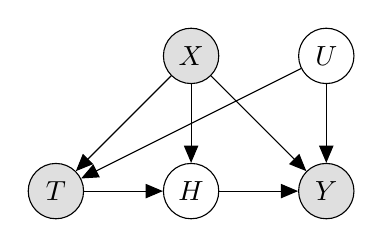
\begin{tikzpicture}

  %
  \node[obs, ]                               (x) {$X$};
  \node[latent, below=of x]                (h) {$H$};
  \node[obs, left=of h]                   (t) {$T$};
  \node[obs, right=of h]                   (y) {$Y$};
  \node[latent, right=of x]                 (u) {$U$};

  %
  \edge {x} {t} ; %
  \edge {x} {h}  ; %
  \edge {x} {y}  ; %
  \edge {t} {h}  ; %
  \edge {h} {y}  ; %
  \edge {u} {t}  ;
  \edge {u} {y}  ;

\end{tikzpicture}}
\caption{\centering \label{fig:confounding:canonical}Canonical\newline confounding}
\end{subfigure}\quad
\begin{subfigure}{0.22\linewidth}
\centering
\scalebox{0.7}{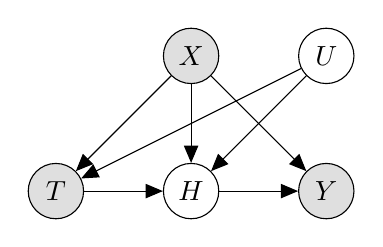
\begin{tikzpicture}

  %
  \node[obs, ]                               (x) {$X$};
  \node[latent, below=of x]                (h) {$H$};
  \node[obs, left=of h]                   (t) {$T$};
  \node[obs, right=of h]                   (y) {$Y$};
  \node[latent, right=of x]                 (u) {$U$};

  %
  \edge {x} {t} ; %
  \edge {x} {h}  ; %
  \edge {x} {y}  ; %
  \edge {t} {h}  ; %
  \edge {h} {y}  ; %
  \edge {u} {t}  ;
  \edge {u} {h}  ;

\end{tikzpicture}}
\caption{\centering \label{fig:confounding:compliance}Response\newline confounding}
\end{subfigure}\quad
\begin{subfigure}{0.22\linewidth}
\centering
\scalebox{0.7}{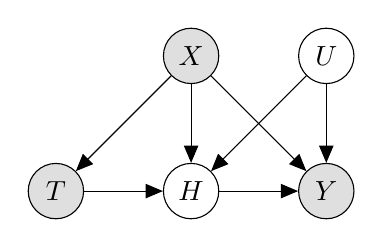
\begin{tikzpicture}

  %
  \node[obs, ]                               (x) {$X$};
  \node[latent, below=of x]                (h) {$H$};
  \node[obs, left=of h]                   (t) {$T$};
  \node[obs, right=of h]                   (y) {$Y$};
  \node[latent, right=of x]                 (u) {$U$};

  %
  \edge {x} {t} ; %
  \edge {x} {h}  ; %
  \edge {x} {y}  ; %
  \edge {t} {h}  ; %
  \edge {h} {y}  ; %
  \edge {u} {h}  ;
  \edge {u} {y}  ;

\end{tikzpicture}}
\caption{\centering \label{fig:confounding:effect}Effect\newline confounding}
\end{subfigure}\quad
\begin{subfigure}{0.22\linewidth}
\centering
\scalebox{0.7}{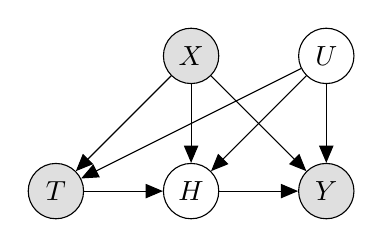
\begin{tikzpicture}

  %
  \node[obs, ]                               (x) {$X$};
  \node[latent, below=of x]                (h) {$H$};
  \node[obs, left=of h]                   (t) {$T$};
  \node[obs, right=of h]                   (y) {$Y$};
  \node[latent, right=of x]                 (u) {$U$};

  %
  \edge {x} {t} ; %
  \edge {x} {h}  ; %
  \edge {x} {y}  ; %
  \edge {t} {h}  ; %
  \edge {h} {y}  ; %
  \edge {u} {t}  ;
  \edge {u} {h}  ;
  \edge {u} {y}  ;

\end{tikzpicture}}
\caption{\centering \label{fig:confounding:total}Total\newline confounding}
\end{subfigure}
\caption{\label{fig:confounding}
The four types of latent confounding in the causal two-groups model.}
\end{figure*}

In this section, we consider how latent confounding impacts statistical inferences in the causal two-groups model. Latent confounding in the C2G model occurs when an unobserved variable $U$ affects two or more of the variables in $\{T, H, Y \}$.  \Cref{fig:confounding} shows the four types of possible latent confounding scenarios.

The key question is whether either of the C2G models proposed above remains \emph{well-specified} under any of these latent confounding scenarios. By well-specified, we mean the observed non-responder and treatment distributions are within the class of probability distributions specified by the modeling assumptions. A well-specified model under latent confounding ensures that integrating out the latent confounder in the untreated group yields the original non-responder distribution and in the treatment group yields the original mixture model,
\begin{equation}
\begin{aligned}
\int p(y | x, u, t=0) p(u) du & = f_0(y \mid x) = p(y | x, h=0, t=1) \, , \\
\int p(y | x, u, t=1) p(u) du &= (1-\pi(x)) f_0(y \mid x) + \pi(x) f_1(y \mid x) \, ,
\end{aligned}
\label{eqn:well-specified}
\end{equation}
where $(\pi, f_0, f_1)$ are specified by the modeling assumptions (i.e. parametric, semi-parametric, or nonparametric). If a model remains well-specified in the presence of latent confounding, statistical inferences will still be valid.

\subsection{Confounding in the additive model}
\label{subsec:confounding:additive}

The additive causal two-groups model requires that the $(f_0, f_1)$ distributions obey \cref{eqn:additive_errors}. Because \cref{eqn:additive_errors} is agnostic to the relationship between $T$ and $H$, it is straightforward to show that the additive causal two groups model remains correctly specified and applicable under response confounding.
\begin{proposition}
\label{prop:compliance-confounding-ac2g}
The additive causal two groups model is robust against response confounding.
\end{proposition}

The story changes when we allow an unobserved random variable to affect the output $Y$. Indeed, even when this variable only affects the conditional means of the non-responder and responder distributions by an additive shift while leaving the noise distribution unchanged, the model is misspecified.

\begin{proposition}
\label{prop:latent-nonrobust-ac2g}
The additive causal two-groups model is misspecified in the presence of an unobserved $U$ such that 
\begin{align*}
Y | X=x, U=u, H=h &=& \mu_{h}(x) + \rho_{h}(u) + \epsilon  \\
\epsilon &\sim& g.
\end{align*}
As a consequence, the additive causal two-groups model is not robust in the presence of canonical, effect, or total confounding.
\end{proposition}


\subsection{Confounding in the nonparametric model}
\label{subsec:confounding:nonparametric}


For the nonparametric method, there are only two modeling assumptions. First, the outcome distribution of the untreated samples must match that of the treated non-responders. Second, the outcome distribution of the treated samples can be written as a mixture model of the form given by \cref{eqn:treatment-mixture}.
The following result shows that this minimalist approach offers an added benefit over the additive model in the form of validity under effect confounding as well as response confounding.

\begin{proposition}
\label{prop:confounding-npc2g}
The nonparametric causal two-groups model is robust against response and effect confounding.
\end{proposition}

The reason why the nonparametric causal two-groups model remains well-specified in the presence of these two types of confounding is that both still allow for $Y \indep T \mid X,  H$. When this conditional independence relationship holds, the non-responder outcome distribution coincides with the untreated outcome distribution. This allows us to write the treatment distribution as the mixture in \cref{eqn:treatment-mixture}, thereby satisfying the conditions of \cref{eqn:well-specified}. When we do not have $Y \indep T \mid X,  H$, we cannot guarantee that the nonparametric causal two-groups model is well-specified, as the following result shows.

\begin{proposition}
\label{prop:canonical-confounding}
The nonparametric causal two-groups model is not robust in the presence of canonical or total confounding.
\end{proposition}

The key to proving \cref{prop:canonical-confounding} is in showing that a canonical confounder $U$ can lead to situations in which the untreated outcome distribution $p(Y \mid X, T=0)$ differs from the treated-but-non-responder outcome distribution $p(Y \mid X, H=0, T=1)$, breaking the fundamental assumptions of the nonparametric causal two-groups model.




\section{Digital Twin for System-level Analysis}
\label{sec:sim}

We develop a detailed digital twin of an area (0.34 km $\times$ 0.28 km) in downtown Philadelphia (shown in Figure~\ref{fig:network}), accurately representing a cellular network operating at millimeter wave frequencies. 
To analyze the network's capacity and coverage, we model only outdoor UE locations, which are uniformly distributed across 1 m $\times$ 1 m grids in outdoor areas.
The radio frequency channels are generated based on ray tracing using parameters provided in Table~\ref{tab:rf_parameters}, along with realistic foliage modeling in the DT and the associated losses. 

The network under consideration consists of 49876 UE locations and $N_C=169$ active cells distributed across 69 sites, meeting the \emph{throughput} target of 50 Mbps for 80\% of UEs in the initial deployment. The same set of cells provides SSB \emph{coverage} to 94\% ($N_{UE}=46884$) of all UEs.

\begin{figure}
\centering
\includegraphics[width=0.9\linewidth]{figs/network.png}
\caption{28GHz network based on Downtown Philadelphia Digital Twin \small{(Map data \copyright  OpenStreetMap contributors, Microsoft, Esri community Maps contributors. Map layers by Esri, markers added for more visibility, license: https://creativecommons.org/licenses/by-sa/2.0/legalcode)}}
    \label{fig:network}
    \vspace{-15pt}
\end{figure}

\begin{table}[]
\begin{center}
%\large
\vspace{10pt}
\begin{tabular}{|c|c|c|}
\cline{1-3} 
\textbf{Parameters}        & \textbf{Cell}         & \textbf{UE}      \\ \cline{1-3} 
{Carrier Frequency}        &  \multicolumn{2}{|c|}{28 GHz}                \\ \cline{1-3}    
{Bandwidth}        &  \multicolumn{2}{|c|}{800 MHz}                \\ \cline{1-3}  
{Antenna array } & 8 row x 24 col  & 2 row x 2 col  \\
{arrangement} & x 2 polarization & x 2 polarization \\ \cline{1-3}
%{Codebook SSB} &  \multicolumn{2}{|c|}{8 Az beams x 4 El beams}  \\ \cline{1-3}
%{SU-MIMO order} & \multicolumn{2}{|c|}{2 }\\    \cline{1-3}  
%{Number of sectors} & 3 & N/A \\   \cline{1-3}  
{Maximum array gain} & 28.15 dBi & 10 dBi \\   \cline{1-3}  
{Body Loss} & N/A & 8 dB \\  \cline{1-3}  
{Implementation margin} & N/A  & 1.9 dB  \\ \cline{1-3}  
{Noise Figure}  & 10 dB & 6.7 dB  \\ \cline{1-3}  
{Cell-edge reliability margin}  & \multicolumn{2}{|c|}{13.2 dB}                \\ \cline{1-3}  
{Foliage loss} &  \multicolumn{2}{|c|}{4 dB/m}                \\ \cline{1-3}  
{Building reflection loss} & \multicolumn{2}{|c|}{6.4 dB}                \\ \cline{1-3} 
\end{tabular}
\caption{Digital-twin parameters}
\label{tab:rf_parameters}
\end{center}
\vspace{-25pt}
\end{table}

\begin{figure*}%[h]
\centering
\begin{subfigure}[b]{0.34\linewidth}
    \includegraphics[width=\linewidth]{figs/baseline_codebook.png}
    \caption{Baseline SSB codebook arrangement.}
    \label{fig:baseline_codebook}
\end{subfigure}
\hfill
\begin{subfigure}[b]{0.31\linewidth}
    \includegraphics[width=\linewidth]{figs/min_snr.png}
    \caption{Minimum SNR along beam directions.}
    \label{fig:min_snr}
\end{subfigure}
\hfill
\begin{subfigure}[b]{0.31\linewidth}
   \includegraphics[width=\linewidth]{figs/sample_hybrid_beams.png}
\caption{Sample of an optimized SSB codebook.}
    \label{fig:sample_hybrid_beam}
\end{subfigure}
\caption{Baseline SSB codebook (a), and opportunities for SSB codebook optimization in (c) for a given cell with a non-uniform coverage (b).}
\label{fig:beam_per_sector}
\vspace{-15pt}
\end{figure*}

The baseline SSB codebook comprises 32 SSB beams, each with a width of 15$^{\circ}$ in azimuth and 7.5$^{\circ}$ in elevation, covering an azimuth span of   120$^{\circ}$ (-60$^{\circ}$ to 60$^{\circ}$) and an elevation span of 30$^{\circ}$ (-30$^{\circ}$ to 0$^{\circ}$), wherein 0$^{\circ}$ elevation is associated with the horizon, and negative values represent angles below the horizon. Figure~\ref{fig:baseline_codebook} shows the arrangement of the beams in the baseline codebook.

For the beam-level optimizations (both local and global), we consider four different types of beams with varying beamwidths in azimuth (BW$_{Az}$) and elevation (BW$_{El}$); Type-1: (BW$_{Az} =$ 15$^{\circ}$, BW$_{El} =$ 7.5$^{\circ}$), 
Type-2: (BW$_{Az} =$ 15$^{\circ}$, BW$_{El} =$ 15$^{\circ}$),
Type-3: (BW$_{Az} =$ 30$^{\circ}$, BW$_{El} =$ 7.5$^{\circ}$), and
Type-4: (BW$_{Az} =$ 30$^{\circ}$, BW$_{El} =$ 15$^{\circ}$).
Figure~\ref{fig:sample_hybrid_beam} shows an example of an SSB codebook comprising beams of different types, optimally selected for a cell with a non-uniform coverage region (as shown in Figure~\ref{fig:min_snr}).
The NES optimizations presented in~\S\ref{sec:system} are solved within the integer solution space using a mixed integer linear program (MILP)~\cite{10.1287/ijoc.2018.0857}.


\begin{table*}[htbp]
    \centering
    \small
    \begin{tabular}{p{14cm}}
     \toprule
\#\#\#  Objective: \\
Generate a 5-day family travel itinerantry that satisfies all specified requirements while adhering to highly fine-grained constraints. The generated itinerary should balance real-time adaptability, strict hard attributes, and semantic soft attributes. \\

\#\#\# User Profile: \\
 - Travelers: 2 adults + 1 child (age 8) \\
 - Budget: $<=$ \$300/day (total \$1,500 for the trip) \\
 - Activity Balance: 70\% educational/cultural experiences, 20\% relaxation, 10\% family-friendly shopping. \\

\#\#\# Hard Attributes: \\
- Activity Scheduling: \\
\quad- Each activity must have a defined start and end time, ensuring there is no overlap between activities. \\
\quad- A break period from 13:00-14:30 is mandatory daily. \\
\quad- Each activity must fit within a 2-hour window unless otherwise specified. \\

- Budget Requirements: \\
\quad- Each day’s total cost (including transportation, food, and activities) must not exceed \$300. \\
\quad- Transportation is limited to metro and walking only, with a maximum of 3 metro rides per day. \\

- Location Constraints: \\
\quad- Must-visit locations: City Zoo (Day 1) and Science Museum (Day 3). \\
\quad- Activities must occur in geographically adjacent areas to minimize walking distance. \\

- Keyword Requirements: \\
\quad- Each day’s description must include specific keywords. For example: \\
\quad- Day 1: “wildlife,” “exploration,” and “interactive learning.” \\
\quad- Day 3: “science,” “innovation,” and “hands-on exhibits.” \\

- Structure Constraints: \\
\quad- Each day’s itinerary must consist of 4 sections: \\
\quad\quad- Morning activity \\
\quad\quad- Break/lunch period \\ 
\quad\quad- Afternoon activity \\
\quad\quad- Evening summary (limited to 50 words) \\

\#\#\# Soft Attributes \\
- Tone and Emotion: \\ 
\quad- Day 1: Use a tone that conveys “excitement and discovery.” \\ 
\quad- Day 3: Use a tone that conveys “curiosity and wonder.” \\
- Language Style: \\ 
\quad- Use descriptive, vivid, and family-friendly language throughout. \\
\quad- Include at least one metaphor or simile per day (e.g., "The Science Museum felt like stepping into the future!"). \\
- Visual Details: \\
\quad- Each activity must include specific sensory details (e.g., "the bright colors of the parrots at the zoo" or "the tinkling sound of water fountains at the park").

- Adaptive Adjustments (Real-time Constraints): \\
\quad- Weather Sensitivity: \\
\quad\quad- If the rain forecast exceeds 60\%, replace outdoor activities with indoor alternatives while keeping the overall tone and keywords intact. \\ 
\quad- Physical Endurance: \\
\quad\quad- If a day’s total walking distance exceeds 10 kilometers, the next day’s activities must reduce walking by 30\%. \\
\quad- Health Responsiveness: \\
\quad\quad- If a health-related issue arises (e.g., fatigue or illness), adjust the itinerary dynamically to: \\
\quad\quad- Reduce activity duration to half. \\ 
\quad\quad- Substitute the activity with a more relaxing or passive option. \\
\bottomrule
    \end{tabular}
    \caption{The complete travel planner case study.}
    \label{tab:travel_planner_case}
\end{table*}

This work identifies signal collapse as a critical bottleneck in one-shot neural network pruning. Performance loss in pruned networks is due to \textbf{signal collapse} in addition to the removal of critical parameters. We propose \textbf{REFLOW} (\textbf{Re}storing \textbf{F}low of \textbf{Low}-variance signals), a simple yet effective method that mitigates signal collapse without computationally expensive weight updates. By focusing on signal preservation, REFLOW highlights the importance of mitigating signal collapse in sparse networks and enables magnitude pruning to match or surpass state-of-the-art one-shot pruning methods such as CHITA, CBS, and WF.

REFLOW consistently achieves state-of-the-art accuracy across diverse architectures, restoring ResNeXt-101 from under 4.1\% to 78.9\% top-1 accuracy at 80\% sparsity on ImageNet. Its lightweight design makes it a practical solution for both research and deployment, delivering high-quality sparse models without the overhead of traditional approaches. These findings challenge the traditional emphasis on weight selection strategies and underscore the critical role of signal propagation for achieving high-quality sparse networks in the context of one-shot pruning.




\section*{Acknowledgments}
{\textcopyright}2025 All rights reserved. The research described in this paper was carried out at the Jet Propulsion Laboratory, California Institute of Technology, under a contract with the National Aeronautics and Space Administration (80NM0018D0004).

{
\small
\bibliography{main}
}


%

\newpage
\appendix

%
%
%

\section{Additional results and details from \Cref{sec:model}}
\subsection{Proof of \cref{thm:unident}}
Consider the following densities over $[0,\infty)$: 
\begin{align*}
    f_0(y) &= \frac{3}{2} e^{-y} - e^{-2y}\\
    f^{(1)}_1(y) &= e^{-y} \\
    f^{(2)}_1(y) &= 2 e^{-2y}.
\end{align*}
It can be readily verified that these are all valid probability densities. Moreover, we can see that $f_0$ is log-concave over its domain since
\[ \frac{d^2}{d y^2} \log f_0(y) = -\frac{2e^y}{3(\frac{2}{3} - e^y)^2} < 0 \, \, \text{ for all 
 } y \geq 0. \]
$f^{(1)}_1$ and $f^{(2)}_1$ are also clearly log-concave since their log-densities are linear.


Suppose that $f_0$ is the observed null distribution. Letting $\pi_1 = \frac{3}{4}$ and $\pi_2 = \frac{1}{4}$, consider the following two observed treatment distributions:
\begin{align*}
f^{(1)}_t(y) &= (1-\pi_1) f_0(y) + \pi_1 f^{(1)}_1(y) \\
f^{(2)}_t(y) &= (1-\pi_2) f_0(y) + \pi_2 f^{(2)}_1(y).
\end{align*}
Using these definitions, we have
\begin{align*}
f^{(1)}_t(y) &= (1-\pi_1) f_0(y) + \pi_1 f^{(1)}_1(y) \\
&= \frac{1}{4} \left( \frac{3}{2} e^{-y} - e^{-2y} \right) + \frac{3}{4} e^{-y} \\
&= \frac{9}{8} e^{-y} - \frac{1}{4} e^{-2y} \\
&= \frac{3}{4} \left( \frac{3}{2} e^{-y} - e^{-2y} \right) + \frac{1}{4} \cdot 2 e^{-y} \\
&= (1-\pi_2) f_0(y) + \pi_2 f^{(2)}_1(y) \\
&= f^{(2)}_t(y).
\end{align*}
Thus, we can conclude that the C2G model is unidentifiable even when both the null distribution and the alternative distribution are restricted to being log-concave.

\subsection{Proof of \cref{prop:normal-identifiability}}

Fix $x$. In \Cref{eqn:two_groups}, we observe distributions $f_0(y \mid x)$ and $f_t(y \mid x)$. Suppose we are given $\mu_0 = \mu_0(x)$, $\mu_1 = \mu_1(x)$, $\mu_2 = \mu_2(x)$, $\sigma_0^2 = \sigma_0^2(x)$, $\sigma_1^2 = \sigma_1^2(x)$, $\sigma_2^2 = \sigma_2^2(x)$,  $\pi_1 = \pi_1(x)$, and $\pi_2 = \pi_2(x)$, where $\pi_1, \pi_2 \in (0,1)$. By translating and scaling the space, we can assume without loss of generality that $\mu_0 = 0$ and $\sigma_0^2 = 1$. Our goal is to show that if
\begin{align}
\label{eqn:normal-identifiability}
(1-\pi_1)\Ncal(y \mid 0, 1) + \pi_1 \Ncal(y \mid \mu_1, \sigma_1^2) = (1-\pi_2)\Ncal(y \mid 0, 1) + \pi_2 \Ncal(y \mid \mu_2, \sigma_2^2) 
\end{align}
for all $y \in \R$, then we must have $\pi_1=\pi_2$, $\mu_1 = \mu_2$, and $\sigma_1^2 = \sigma_2^2$. There are two cases to consider here.

\paragraph{Case 1: $\pi_1 = \pi_2$.} In this case, we immediately have
\[ \Ncal(y \mid \mu_1, \sigma_1^2) = \Ncal(y \mid \mu_2, \sigma_2^2) \]
for all $y \in \R$. Taking the first moment of both sides, we have $\mu_1 = \mu_2$. Conditioned on this fact, we can calculate the variance of both sides to conclude $\sigma_1^2 = \sigma_2^2$. 

\paragraph{Case 2: $\pi_1 \neq \pi_2$.} In this case, we will come to a contradiction. Assume without loss of generality that $\pi_1 > \pi_2$. Letting $\beta = \frac{\pi_2}{\pi_1 - \pi_2} > 0$, we can rearrange \cref{eqn:normal-identifiability} to get
\[ \Ncal(y \mid 0, 1) = (1+\beta) \Ncal(y \mid \mu_1, \sigma_1^2) - \beta \Ncal(y \mid \mu_2, \sigma_2^2).  \]
Multiplying both sides by $e^{ty}$ and integrating $y \in \R$, the moment generating function of the normal distribution gives us
\begin{align}
\label{eqn:normal-identifiability-mgf}
\exp\left( t^2/2 \right)
= (1+\beta)\exp\left( \mu_1 t + \sigma_1^2 t^2/2 \right) - \beta \exp\left( \mu_2 t + \sigma_2^2 t^2/2 \right)   
\end{align}
for all $t \in \R$. We will analyze \cref{eqn:normal-identifiability-mgf} in the limit as $t\rightarrow \infty$.

Observe first that we must have $\sigma_2^2 \leq \sigma_1^2$, since otherwise as $t\rightarrow \infty$, the RHS of \cref{eqn:normal-identifiability-mgf} tends to $-\infty$ while the LHS is positive. 

Now consider the case where $\sigma_2^2 < \sigma_1^2$. Multiplying \cref{eqn:normal-identifiability-mgf} through by $e^{-\mu_1 t - \sigma_1^2 t^2/2}$, we have
\[ \exp\left( -\mu_1 t - (\sigma_1^2 - 1) t^2/2 \right) = 1+\beta - \beta \exp\left( (\mu_2 - \mu_1) t - (\sigma_1^2 -\sigma_2^2) t^2/2 \right).  \]
As $t\rightarrow \infty$, the RHS tends to $1 + \beta$. On the other hand, the LHS must tend to either 0 or $+\infty$. Thus we must have $\sigma_1^2 = \sigma_2^2$. In which case, we can rearrange \cref{eqn:normal-identifiability-mgf} to obtain
\[ 1 = \left[(1+\beta)\exp(\mu_1 t) - \beta \exp(\mu_2 t) \right] \exp\left( (\sigma_1^2 - 1)t^2/2 \right). \]
If $\sigma_1^2 < 1$, then the RHS must tend to 0. If $\sigma_1^2 > 1$, then the RHS must tend to $\pm \infty$. Thus, we can conclude $\sigma_1^2 = 1$, and the above equation becomes
\[ 1 = \left[(1+\beta)\exp(\mu_1 t) - \beta \exp(\mu_2 t) \right]. \]
The only way for this to hold for all $t$ is if $\mu_1 = \mu_2=0$.

\section{Additional results and details from \Cref{sec:additive}}
\subsection{Proof of \cref{thm:additive-identify}}

For any $x$, observe that we can shift the space by $\mu_0(x)$ so that the model in \Cref{eqn:additive_errors} becomes
\begin{align*}
f_0(y \mid x) &= g(y) \\
f_1(y \mid x) &= g(y - \tau(x)).
\end{align*}
In this case, the observable distributions are the null distribution $f_0 = g$ and the treatment distribution
\[ f_t(y \mid x) = (1-\pi(x)) g(y) + \pi(x) g(y - \tau(x)).  \]
Fixing a particular $x$, the identifiability of \Cref{eqn:additive_errors} can be restated as follows.

\begin{theorem}[Restatement of \cref{thm:additive-identify}]
\label{thm:additive-identify-restate}
Let $g$ denote a probability density function over $\R$. For $\pi \in (0,1)$, $\tau \in \R$, define the density function 
\[ f(y ; \pi, \tau) = (1- \pi) g(y) + \pi g(y-\tau). \]
Then the family of densities $\{f(y ; \pi, \tau) \,  \mid \, \pi \in (0,1), \tau \in \R \setminus \{ 0\} \}$ is identifiable.
\end{theorem}
    
We begin by recalling the characteristic function of a probability distribution. If $g$ is a probability distribution over $\R$, then its characteristic function is given by
\[ \varphi_g(\omega) = \E_{X\sim g}\left[ e^{-i \omega X} \right] = \int_{-\infty}^\infty g(x) e^{-i \omega x} \, dx,  \]
where $\omega \in \R$ and the integral is only well-defined when $g$ is a probability density function. We will make use of the following elementary property of the characteristic function.

\begin{lemma}
\label{lem:charfun-property}
For any probability density function $g$, there exists a value $\omega_0 > 0$ such that $|\varphi_g(\omega)| > 0$ for all $\omega \in [0, \omega_0]$.
\end{lemma}
\begin{proof}
This follows directly from the fact that $\varphi_g$ is uniformly continuous on $\R$ and $\varphi_g(0) = 1$ \citep{resnick:2013:probability}.
\end{proof}

With this tool in hand, we turn to the proof of \Cref{thm:additive-identify-restate}.

\begin{proof}[Proof of \Cref{thm:additive-identify-restate}]
Let $\pi_1, \pi_2 \in (0,1)$ and $\tau_1, \tau_2 \in \R \setminus \{ 0 \}$ be parameters such that $f(y;\pi_1, \tau_1) = f(y;\pi_2, \tau_2)$. Our goal is to show that we must have $\pi_1 = \pi_2$ and $\tau_1 = \tau_2$. We consider two cases.


\paragraph{Case 1: $\pi_1 = \pi_2$.} In this case, we must have
\begin{align*}
0 &= f(y;\pi_1, \tau_1) - f(y;\pi_2, \tau_2) \\
&= (1- \pi_1) g(y) + \pi_1 g(y-\tau_1) - (1- \pi_2) g(y) - \pi_2 g(y-\tau_2) \\
&= \pi_1 g(y-\tau_1) - \pi_1 g(y - \tau_2)
\end{align*}
for all $y \in \R$. Multiplying through by $e^{i \omega y}/\pi_1$ and integrating over $\R$, we have
\begin{align*}
0 &= \int_{-\infty}^\infty g(y-\tau_1) e^{i \omega y} \, dy - \int_{-\infty}^\infty g(y-\tau_2) e^{i \omega y} \, dy \\
&= \int_{-\infty}^\infty g(y) e^{i \omega (y+\tau_1)} \, dy - \int_{-\infty}^\infty g(y) e^{i \omega (y+\tau_2)} \, dy \\
&= \varphi_g(\omega) e^{i\omega \tau_1} - \varphi_g(\omega) e^{i\omega \tau_2},
\end{align*}
which holds for all $\omega \in \R$. Invoking \Cref{lem:charfun-property}, there is a value a value $\omega_0 > 0$ such that $|\varphi_g(\omega)| > 0$ for all $\omega \in [0, \omega_0]$. Plugging $\omega = \min \left( \omega_0, \frac{\pi}{|\tau_1 - \tau_2|}\right)$ into the above and dividing by $\varphi_g(\omega)$, we can rearrange to observe
\[ e^{i \omega (\tau_1 - \tau_2)} = 1. \]
This can only be true if $\omega (\tau_1 - \tau_2) = 2 \pi n$ for some $n \in \Z$. By our choice of $\omega$, it must be the case that $\tau_1 = \tau_2$.

\paragraph{Case 2: $\pi_1 \neq \pi_2$.} Here we will reach a contradiction. Assume without loss of generality that $\pi_1 < \pi_2$. Then we have
\begin{align*}
0 &= f(y;\pi_1, \tau_1) - f(y;\pi_2, \tau_2) \\
&= (1- \pi_1) g(y) + \pi_1 g(y-\tau_1) - (1- \pi_2) g(y) - \pi_2 g(y-\tau_2) \\
&= (\pi_2 - \pi_1) g(y) + \pi_1 g(y-\tau_1) - \pi_2 g(y-\tau_2)
\end{align*}
for all $y \in \R$. Multiplying through by $e^{i \omega y}$ and integrating over $\R$, we have
\begin{align*}
0 &= (\pi_2 - \pi_1) \int_{-\infty}^\infty g(y) e^{i \omega y} \, dy + \pi_1\int_{-\infty}^\infty g(y-\tau_1) e^{i \omega y} \, dy - \pi_2 \int_{-\infty}^\infty g(y-\tau_2) e^{i \omega y} \, dy \\
&= (\pi_2 - \pi_1) \varphi_g(\omega) + \pi_1 \varphi_g(\omega) e^{i\omega \tau_1} - \pi_2 \varphi_g(\omega) e^{i\omega \tau_2},
\end{align*}
for all $\omega \in \R$. Invoking \Cref{lem:charfun-property} again, we have $|\varphi_g(\omega)| > 0$ for all $\omega \in [0, \omega_0]$.  Taking $\omega = \min( \omega_0, \frac{\pi}{|\tau_1|})$, we divide through by $\varphi_g(\omega) \pi_2$ and rearrange to get
\[ e^{i \omega \tau_2} = 1 - \frac{\pi_1}{\pi_2} + \frac{\pi_1}{\pi_2} e^{i \omega \tau_1} = 1 - p + p e^{i \omega \tau_1},\]
where $p \in (0, 1/2)$. Taking magnitudes of both sides, we have
\begin{align*}
1 = \left| e^{i \omega \tau_2} \right| &= \left| 1 - p + p e^{i \omega \tau_1} \right| \\
&= \left| 1 - p + p( \cos(\omega \tau_1) + i \sin(\omega \tau_1)) \right| \\
&= \sqrt{ (1 - p + p \cos(\omega \tau_1))^2 + p^2 \sin^2(\omega \tau_1) } \\
&= \sqrt{ 1 - 2p(1-p)(1-\cos(\omega \tau_1))} < 1,
\end{align*}
where the last line follows from our choice of $\omega$. Thus, we have reached a contradiction.
\end{proof}
    



\subsection{Proof of \Cref{thm:additive-fdr}}

We require the following result showing that we our posterior estimates are accurate.

\begin{lemma}
\label{lem:additive-posterior-approximation}
Suppose that the conditions of \Cref{thm:additive-fdr} hold. Then for all $i=1,\ldots, n$, the absolute difference
\[ \left|\frac{(1-{\pi}(x_i)) {g}(y_i - \mu_0(x_i))}{(1-{\pi}(x_i)) {g}(y_i - \mu_0(x_i)) + {\pi}(x_i) {g}(y_i - \mu_1(x_i))} - \frac{(1-\hat{\pi}(x_i)) \hat{g}(y_i - \hat{\mu_0}(x_i))}{(1-\hat{\pi}(x_i)) \hat{g}(y_i - \hat{\mu_0}(x_i)) + \hat{\pi}(x_i) \hat{g}(y_i - \hat{\mu_1}(x_i))} \right| \]
is bounded above by $\frac{2U(U+2(\lambda + 1))}{L^2} \epsilon. $
\end{lemma}
\begin{proof}
Pick an index $i=1, \ldots, n$. We use the following notation
\begin{align*}
g_0 = {g}(y_i - \mu_0(x_i)), \, 
g_1 = {g}(y_i - \mu_1(x_i)), \,
\hat{g_0} = \hat{g}(y_i - \hat{\mu_0}(x_i)), \,
\hat{g_1} = \hat{g}(y_i - \hat{\mu_1}(x_i)).
\end{align*}
The smoothness of $g$ combined with the approximation factor of $\hat{\mu_0}$ implies
\[ |g_0 - \hat{g_0}| \leq |{g}(y_i - \mu_0(x_i)) - {g}(y_i - \hat{\mu_0}(x_i))| + |{g}(y_i - \hat{\mu_0}(x_i)) - \hat{g}(y_i - \hat{\mu_0}(x_i))| \leq \epsilon(\lambda + 1).\]
A symmetrical argument shows the same holds for $|g_1 - \hat{g_1}|$. Thus, we can conclude the following
\begin{align*}
|\pi(x_i) g_1 - \hat{\pi}(x_i)\hat{g}_1| &\leq \epsilon(U + 2(\lambda + 1) ) \\
|(1-\pi(x_i)) g_0 - (1-\hat{\pi}(x_i))\hat{g}_0 | &\leq \epsilon(U + 2(\lambda + 1) ) \\
(1-\hat{\pi}(x_i))\hat{g}_0  + \hat{\pi}(x_i)\hat{g}_1 &\geq L/2 \\ 
(1-{\pi}(x_i)){g}_0  + {\pi}(x_i){g}_1 &\leq U.
\end{align*}
Using the shorthand $a = (1-\pi(x_i)) g_0$, $\hat{a} = (1-\hat{\pi}(x_i))\hat{g}_0$, $b = \pi(x_i) g_1$, and $\hat{b} = \hat{\pi}(x_i)\hat{g}_1$, we have
\begin{align*}
\left| \frac{a}{a+b} - \frac{\hat{a}}{\hat{a} + \hat{b}} \right| 
&= \left|\frac{\hat{a}b - \hat{b}a}{(a+b)(\hat{a} + \hat{b})} \right| \\
&\leq \frac{2}{L^2}\left|\hat{a}b - \hat{b}a\right| \\
&\leq \frac{2}{L^2} (a+b) \epsilon (U + 2) = \frac{2U(U+2(\lambda + 1))}{L^2} \epsilon. \qedhere
\end{align*}

\end{proof}


Our next lemma is an elementary result concerning sums of probabilities.
\begin{lemma}
\label{lem:prob-subset-sum}
Let $p_1, \hat{p}_1, p_2, \hat{p_2}, \ldots, p_n, \hat{p}_n, \alpha, \delta \in [0,1]$ such that $\left|p_i - \hat{p_i}\right| \leq \delta$ for all $i=1,\ldots, n$. Let $V, \hat{V} \subset \{1,\ldots, n\}$ be the largest subsets such that 
\[ \frac{1}{|V|} \sum_{i\in V} p_i \leq \alpha - \delta \text{ and }  \frac{1}{|\hat{V}|} \sum_{i\in \hat{V}} \hat{p}_i \leq \alpha .  \]
Then 
\[\sum_{i\in \hat{V}} 1 - {p}_i \geq \frac{1 - \alpha - \delta}{1 - \alpha + \delta + 1/(|V|+1)}\sum_{i\in {V}} 1 - {p}_i.\]
\end{lemma}
\begin{proof}
Observe first that $|\hat{V}| \geq |V|$, since 
\[ \frac{1}{|{V}|} \sum_{i\in {V}} \hat{p}_i \leq \frac{1}{|{V}|} \sum_{i\in {V}} ({p}_i + \delta) \leq \alpha. \]
Now observe that
\[ \sum_{i\in \hat{V}} 1 - {p}_i \geq \sum_{i\in \hat{V}} 1 - \hat{p}_i - \delta = |\hat{V}|(1 - \alpha - \delta) \geq |{V}|(1 - \alpha - \delta). \]
On the other hand, by considering adding a single element to $V$, we have
\[  \frac{1}{|V|} \sum_{i \in V} p_i \geq \alpha - \delta - \frac{1}{|V|+1}.  \]
Thus,
\[ \sum_{i\in {V}} 1 - {p}_i \leq |V|\left( 1 - \alpha + \delta + \frac{1}{|V|+1} \right). \]
Taking ratios completes the proof.
\end{proof}


We now turn to the proof of \cref{thm:additive-fdr}.

\begin{proof}[Proof of \cref{thm:additive-fdr}]
Let $(x_1, y_1, t_1, h_1), \ldots, (x_n, y_n, t_n, h_n)$ denote the samples from \cref{eqn:additive_errors} (where $h_1,\ldots, h_n$ are unobserved). From the structure of \cref{eqn:additive_errors}, we have that, conditioned on $(x_1, y_1, t_1), \ldots, (x_n, y_n, t_n)$, the random variables $\ind[h_i = 0]$ are Bernoulli random variables with biases $p_i = \pr(h_i = 0 \mid x_i, y_i, t_i)$.

From \Cref{lem:additive-posterior-approximation}, we have that
\[ \left| \hat{w}_i - \pr(H=0 \mid x_i, y_i, t_i=1)\right| \leq \frac{2U(U+2(\lambda + 1))}{L^2} \epsilon \]
for all $i=1,\ldots, n$. If $S$ is a set of indices satisfying $t_i=1$ for all $i \in S$ and $\frac{1}{|S|} \sum_{i\in S} \hat{w}_i \leq \alpha$, then
\begin{align*}
\E \left[ \frac{1}{|S|} \sum_{i \in S} \ind[h_i = 0] \mid (x_1, y_1, t_1), \ldots, (x_n y_n, t_n) \right] 
&= \frac{1}{|S|} \sum_{i \in S} \E\left[ \ind[h_i = 0] \mid (x_1, y_1, t_1), \ldots, (x_n y_n, t_n) \right] \\
&=  \frac{1}{|S|} \sum_{i \in 
S} \hat{w}_i +\frac{2U(U+2(\lambda + 1))}{L^2} \epsilon \\
&\leq \alpha + \frac{2U(U+2(\lambda + 1))}{L^2} \epsilon. 
\end{align*}

To prove the power statement, observe that the Bayes' optimal procedure is to choose the largest set $V$ such that $ \frac{1}{|V|}\sum_{i \in V} p_i \leq \alpha$. Then the power conclusion follows directly from \cref{lem:prob-subset-sum} with $\delta = \frac{2U(U+2(\lambda + 1))}{L^2} \epsilon$.
\end{proof}

\section{Additional results and details from \Cref{sec:kernel_generalized}}
\subsection{Proof of \cref{lem:conservative-pi}}
Suppose there exist distributions $\pi$, $f_0$, $f_1$ such that
\begin{align*}
p(y \mid x, t=0) &:= f_0(y \mid x), \text{ and } \\
p(y \mid x, t=1) &:= f_t(y \mid x) = (1-\pi(x)) f_0(y \mid x) + \pi(x) f_1(y \mid x).
\end{align*}
Pick any $x$. Observe that if $\pi(x)=0$, then the corresponding $\pi^\star(x) = 0$ and the lemma conclusion trivially holds. Thus, we may assume $\pi(x) > 0$, in which case we have by rearrangement:
\[ f_1(y \mid x) = \frac{1}{\pi(x)} \left( f_t(y \mid x) - f_0(y \mid x) \right) + f_0(y \mid x). \]
As a probability density, $f_1(y \mid x) \geq 0$, which implies
\[  \pi(x) \geq 1 - \frac{f_t(y \mid x)}{f_0(y \mid x)}. \]
Since the above holds for all $y$, we therefore must have 
\[  \pi(x) \geq 1 - \min_y \frac{f_t(y \mid x)}{f_0(y \mid x)} = \pi^\star(x). \]


To prove the second part of the lemma, let $x$ be a point and $\hat{\pi}$ be a function satisfying $1 \geq \hat{\pi}(x) \geq \pi^\star(x) > 0$. Then define
\[ f_1^{\hat{\pi}}(y \mid x) = \frac{1}{\hat{\pi}(x)} \left( f_t(y \mid x) - f_0(y \mid x) \right) + f_0(y \mid x). \]
By definition of $\pi^\star$, we have $f_1^{\hat{\pi}}(y \mid x) \geq 0$. Moreover, integrating the right hand side over $y$ shows that $f_1^{\hat{\pi}}(y \mid x)$ integrates to 1. Thus, $f_1^{\hat{\pi}}(y \mid x)$ is a proper density. Rearrangement shows that
\[ f_t(y \mid x) = (1-\hat{\pi}(x)) f_0(y \mid x) + \hat{\pi}(x) f_1^{\hat{\pi}}(y \mid x). \]

\subsection{Proof of \Cref{thm:general-fdr}}

To prove \Cref{thm:general-fdr} we first need to prove some lemmas. The first lemma shows that under the conditions of \Cref{thm:general-fdr},  we can estimate $\pi^\star$ accurately.

\begin{lemma}
\label{lem:w_star-estimate}
Let $\epsilon, L, U > 0$ be given. Suppose the following holds for all $i=1, \ldots n$ and $y \in \Ycal$:
\begin{itemize}
    \item[(i)] $L \leq f_t(y \mid x_i), f_0(y \mid x_i) \leq U$,
    \item [(ii)] $|f_t(y \mid x_i) - \hat{f}_t(y \mid x_i)| \leq \epsilon$, and
    \item[(iii)] $|f_0(y \mid x_i) - \hat{f}_0(y \mid x_i)| \leq \epsilon$.
\end{itemize}
If $\epsilon \leq L/2$, then $|\hat{\pi}^\star(x_i) - \pi^\star(x_i)| \leq \frac{8 U \epsilon}{L^2}$ for all $i=1,\ldots, n$, where
$ \hat{\pi}^\star(x) = 1 - \min_y \frac{\hat{f}_t(y \mid x)}{\hat{f}_0(y \mid x)} .$
\end{lemma}
\begin{proof}
Pick some index $i$, and let $x = x_i$. Let $y = \argmin_y \frac{f_t(y \mid x)}{f_0(y \mid x)}$ and $\hat{y} = \argmin_y \frac{\hat{f}_t(y \mid x)}{\hat{f}_0(y \mid x)}$. Then we can write
\begin{align*}
\hat{\pi}^\star(x) - \pi^\star(x)
&=  \frac{f_t(y \mid x)}{f_0(y \mid x)} - \frac{\hat{f}_t(\hat{y} \mid x)}{\hat{f}_0(\hat{y} \mid x)}  \\
&= \frac{f_t(y \mid x)}{f_0(y \mid x)} - \frac{f_t(\hat{y} \mid x)}{f_0(\hat{y} \mid x)} + \frac{f_t(\hat{y} \mid x)}{f_0(\hat{y} \mid x)} - \frac{\hat{f}_t(\hat{y} \mid x)}{\hat{f}_0(\hat{y} \mid x)} \\
&\leq \frac{f_t(\hat{y} \mid x)}{f_0(\hat{y} \mid x)} - \frac{\hat{f}_t(\hat{y} \mid x)}{\hat{f}_0(\hat{y} \mid x)} \\
&= \frac{f_t(\hat{y} \mid x) \hat{f}_0(\hat{y} \mid x) - f_0(\hat{y} \mid x)\hat{f}_t(\hat{y} \mid x)}{f_0(\hat{y} \mid x) \hat{f}_0(\hat{y} \mid x)} \\
&\leq \frac{(\hat{f}_t(\hat{y} \mid x) + \epsilon )(f_0(\hat{y} \mid x) + \epsilon) - f_0(\hat{y} \mid x)\hat{f}_t(\hat{y} \mid x)}{f_0(\hat{y} \mid x) \hat{f}_0(\hat{y} \mid x)} \\
&\leq \frac{2\epsilon(U + \epsilon)}{L^2/2} \leq \frac{8U\epsilon}{L^2}.
\end{align*}
The first inequality comes from the definition of $y$, the second inequality comes from Assumptions (ii) and (iii), and the last two inequalities follow from Assumption (i). A symmetric line of reasoning that demonstrates $\pi^\star(x) - \hat{\pi}^\star(x) \leq \frac{8U\epsilon}{L^2}$ completes the proof.
\end{proof}

Our second lemma shows that the posterior estimate in \cref{eqn:generalized_w_estimate} is close to the ground truth value.

\begin{lemma}
\label{lem:posterior-approximation}
Let $\epsilon, L, U > 0$ be given. Suppose the following holds for all $i=1, \ldots n$ and $y \in \Ycal$:
\begin{itemize}
    \item[(i)] $L \leq f_t(y \mid x_i), f_0(y \mid x_i) \leq U$,
    \item [(ii)] $|f_t(y \mid x_i) - \hat{f}_t(y \mid x_i)| \leq \epsilon$, and
    \item[(iii)] $|f_0(y \mid x_i) - \hat{f}_0(y \mid x_i)| \leq \epsilon$.
\end{itemize}
If $\epsilon \leq \min (L/2, 1)$, then for all $i=1,\ldots, n$,
\[ \left|\frac{(1 - \pi^\star(x_i)) f_0(y_i \mid x_i)}{f_t(y_i \mid x_i)} - \frac{(1 - \hat{\pi}^\star(x_i)) \hat{f}_0(y_i \mid x_i)}{\hat{f}_t(y_i \mid x_i)} \right| \leq \frac{8U}{L^2} \left( 1 + \frac{12U}{L^2}\right) \epsilon.  \]
\end{lemma}
\begin{proof}
Let $x=x_i$, $y = y_i$. Then we have
\begin{align*}
&\frac{(1 - \pi^\star(x)) f_0(y \mid x)}{f_t(y \mid x)} - \frac{(1 - \hat{\pi}^\star(x)) \hat{f}_0(y \mid x)}{\hat{f}_t(y \mid x)}\\
&\hspace{3em}= \frac{(1 - \pi^\star(x)) f_0(y \mid x) \hat{f}_t(y \mid x) - (1 - \hat{\pi}^\star(x)) \hat{f}_0(y \mid x)f_t(y \mid x)}{f_t(y \mid x)\hat{f}_t(y \mid x)} \\
&\hspace{3em}\leq \frac{ ((1 - \hat{\pi}^\star(x)) + \frac{8U\epsilon}{L^2}) (\hat{f}_0(y \mid x) + \epsilon)(f_t(y \mid x) + \epsilon)- (1 - \hat{\pi}^\star(x)) \hat{f}_0(y \mid x)f_t(y \mid x)}{f_t(y \mid x)\hat{f}_t(y \mid x)} \\
&\hspace{3em}\leq \frac{(U + \epsilon)\epsilon + U\epsilon + \epsilon^2 + \frac{8U^2 \epsilon}{L^2}(U+\epsilon) + \frac{8U \epsilon}{L^2}\epsilon^2 (U + \epsilon) + \frac{8U^2 \epsilon^2}{L^2} + \frac{8U \epsilon^3}{L^2} }{L^2/2} \\
&\hspace{3em}\leq \frac{8U}{L^2} \left( 1 + \frac{12U}{L^2}\right) \epsilon. 
\end{align*}
Here, we have used \cref{lem:w_star-estimate} in the first inequality.
\end{proof}

We now turn to the proof of \cref{thm:general-fdr}, which is nearly identical to the proof of \cref{thm:additive-fdr}.

\begin{proof}[Proof of \cref{thm:general-fdr}]
Let $(x_1, y_1, t_1, h_1), \ldots, (x_n, y_n, t_n, h_n)$ denote draws from \cref{eqn:two_groups} (where $h_1,\ldots, h_n$ are unobserved). From the structure of \cref{eqn:two_groups}, we have that, conditioned on $(x_1, y_1, t_1), \ldots, (x_n, y_n, t_n)$, the random variables $\ind[h_i = 0]$ are Bernoulli random variables with biases $p_i = \pr(h_i = 0 \mid x_i, y_i, t_i)$.

From \Cref{lem:posterior-approximation}, we have that
\[\hat{w}_i \leq \pr(H=0 \mid x_i, y_i, t_i=1) + \frac{8U}{L^2} \left( 1 + \frac{12U}{L^2}\right) \epsilon \]
for all $i=1,\ldots, n$. If $S$ is a set of indices satisfying $t_i=1$ for all $i \in S$ and $\frac{1}{|S|} \sum_{i\in S} \hat{w}_i \leq \alpha$, then
\begin{align*}
\E \left[ \frac{1}{|S|} \sum_{i \in S} \ind[h_i = 0] \mid (x_1, y_1, t_1), \ldots, (x_n y_n, t_n) \right] 
&= \frac{1}{|S|} \sum_{i \in S} \E\left[ \ind[h_i = 0] \mid (x_1, y_1, t_1), \ldots, (x_n y_n, t_n) \right] \\
&=  \frac{1}{|S|} \sum_{i \in 
S} \hat{w}_i + \frac{8U}{L^2} \left( 1 + \frac{12U}{L^2}\right) \epsilon \\
&\leq \alpha + \frac{8U}{L^2} \left( 1 + \frac{12U}{L^2}\right)\epsilon.
\end{align*}
To prove the power statement, we first observe that the Bayes' optimal procedure is to select the largest set such that $\frac{1}{|V|} \sum_{i\in V} p_i \leq \alpha$, where $p_i = \pr(h_i = 0 \mid x_i, y_i, t_i)$ is formed using the prior $\pi^\star$ from \cref{lem:conservative-pi}. Then \cref{lem:prob-subset-sum} finishes the argument.
\end{proof}

\section{Additional results and details from \Cref{sec:confounding}}
%
\subsection{Proof of \cref{prop:compliance-confounding-ac2g}}

The full compliance confounding additive causal two-groups model is as follows.

\begin{align*}
T |  X=x, U=u &\sim& \textnormal{Bern}(\phi(x,u))  \\
H | X=x, U=u, T=0 &=& 0  \\
H | X=x, U=u, T=1 &\sim& \textnormal{Bern}(\pi(x,u))  \\
Y | X=x, H=h &=& \mu_{h}(x) + \epsilon  \\
\epsilon &\sim& g.
\end{align*}

To show that the additive causal two-groups model is well-specified, observe that we still have
\[ p(Y = y \mid X=x, T=0 ) 
= p(Y = y \mid X=x, H=0 ) 
=  {g}(y - {\mu}_0(x)). \]
Thus, all that remains to be shown is that when we marginalize over $U$, we can write out
\[ p(Y = y \mid X=x, T=1) =  (1-\pi(x)) {g}(y - {\mu}_0(x)) + \pi(x) {g}(y - \mu_1(x)) .\]
Working it out,
\begin{align*}
p(Y = y \mid X=x, T=1) &= \sum_{h =0}^1 p(H=h \mid X=x, T=1) p(Y = y \mid X=x, H=h) \\
&= \sum_{h =0}^1 p(H=h \mid X=x, T=1) g(y - \mu_h(x)).
\end{align*}
Marginalizing over $U$, we have
\begin{align*}
p(H=1 \mid X=x, T=1) &= \int p(U = u \mid X=x, T=1) p(H = 1 \mid X=x, U=u, T=1) \, du \\
&= \int p(U = u \mid X=x, T=1) \pi(x,u) \, du \\
&=: \pi(x),
\end{align*}
where we have simply defined $\pi(x)$ in the last line. Putting it all together gives us the desired result.


\subsection{Proof of \cref{prop:latent-nonrobust-ac2g}}

Consider the following model.
\begin{align*}
H \mid X=x, T=1 &\sim& \textnormal{Bern}(\pi(x)) \\ 
Y \mid X=x, U=u, H=0 &\sim& \mu_0(x) + u + \epsilon \\ 
Y \mid X=x, U=u, H=1 &\sim& \mu_1(x) + \epsilon \\ 
U, \epsilon &\sim& \Ncal(0,1).
\end{align*}
Marginalizing over $U$ and $\epsilon$, we have
\begin{align*}
Y \mid X=x, H=0 &\sim& \Ncal(\mu_0(x),2) \\ 
Y \mid X=x, H=1 &\sim& \Ncal(\mu_1(x),1).
\end{align*}
As the above have different standard deviations, this model cannot be rewritten in the form of \cref{eqn:additive_errors}. Thus, the additive causal two-groups model is misspecified here.
\subsection{Proof of \cref{prop:confounding-npc2g}}

We need to show that $p(Y \mid X, T=1)$ can be written as a mixture model as in \cref{eqn:treatment-mixture}. This can be done by making use of the condition $Y \indep T \mid X, H$:
\begin{align*}
p(Y = y \mid X=x, T=1) &= \sum_{h=0}^1 p(H=h \mid X=x, T=1) p(Y = y \mid X=x, T=1, H=h) \\
&= \sum_{h=0}^1 p(H=h \mid X=x, T=1) p(Y = y \mid X=x, H=h) \\
&= (1-\pi(x)) f_0(y \mid x) + \pi(x) f_1(y \mid x).
\end{align*}
Here, we have simply defined $\pi(x) = p(H=1 \mid X=x, T=1)$, $f_0(y \mid x) = p(Y = y \mid X=x, H=0)$, and $f_1(y \mid x) = p(Y = y \mid X=x, H=1)$. \qed

\subsection{Proof of \cref{prop:canonical-confounding}}

We will make use of the following lemma.

\begin{lemma}
\label{lem:general-latent-confounding}
Let $\Dcal$ and $\Dcal'$ be two distributions. For random variables $X, Y, H, T, U$, there is a choice of distributions for $U$, $Y|X,H,U$, $T|X,U$, and $H|X,T$ such that
\begin{enumerate}
\item $X, Y, H, T, U$ obey the canonical confounding graphical model,
\item $\pr(T=1 \mid X) = 1/2$ [no treatment overlap violations],
\item $\pr(H=0 \mid X, T=0) = 1$ [all untreated are non-responders], 
\item $\pr(H=1 \mid X, T=1) = 1/2$ [no responder overlap violations], 
\item $Y \mid X, T=0 \sim \Dcal'$, and
\item $Y \mid X, H=0, T=1 \overset{d}{=} Y \mid X, H=1, T=1 \overset{d}{=} Y \mid X, T=1 \sim \Dcal$ [matching responder and non-responder distributions].
\end{enumerate}
\end{lemma}
\begin{proof}
Our conditional distributions will be independent of $X$, so we will drop $X$ going forward. We make the following choices for the conditional distributions
\begin{align*}
Y \mid  H=0, U=0 &\sim \Dcal \\
Y \mid H=0, U=1 &= \Dcal' \\
Y \mid H=1, U=0 &= \Dcal \\
Y=1 \mid H=1, U=1 &= \Dcal' \\
\pr(T=1 \mid U=0) &= 1 \\ 
\pr(T = 1 \mid U=1) &= 0 \\ 
\pr(H=1 \mid T=1) &= 1/2 \\
\pr(H=0 \mid T=0) &= 1 \\
\pr(U=1) &= 1/2.
\end{align*}
Then we can work out the following
\begin{align*}
\pr(T=1) &= \pr(U=1)\pr(T = 1 \mid U=1) + \pr(U=0)\pr(T = 1 \mid U=0) = 1/2 \\
\pr(U=1 \mid H, T=1) &= \pr(U=1 \mid T=1) \\
&= \frac{\pr(T=1 \mid U=1)\pr(U=1)}{\pr(T=1 \mid U=1)\pr(U=1) + \pr(T=1 \mid U=0)\pr(U=0)} = 0 \\
\pr(U=1 \mid H, T=0) &= \pr(U=1 \mid T=0) \\
&= \frac{\pr(T=0 \mid U=1)\pr(U=1)}{\pr(T=0 \mid U=1)\pr(U=1) + \pr(T=0 \mid U=0)\pr(U=0)} = 1 \\
\pr(U=0 \mid H, T=1) &= 1 \\
\pr(U=0 \mid H, T=0) &= 0.
\end{align*}
And so we have
\begin{align*}
\pr(Y=y | H=1, T=1) &= \pr(Y=y \mid H=1, U=0, T=1) \pr(U=0 \mid H=1, T=1) \\
&\hspace{2em} +  \pr(Y=y \mid H=1, U=1, T=1) \pr(U=1 \mid H=1, T=1) \\
&= \pr(Y=y \mid H=1, U=0) \pr(U=0 \mid H=1, T=1) \\
&\hspace{2em} +  \pr(Y=y \mid H=1, U=1) \pr(U=1 \mid H=1, T=1) \\
&= \pr(Y=y \mid H=1, U=0).
\end{align*}
Thus, $Y \mid H=1, T=1 \sim \Dcal$. Similarly, we have
\begin{align*}
\pr(Y=y | H=0, T=1) &= \pr(Y=y \mid H=0, U=0, T=1) \pr(U=0 \mid H=0, T=1) \\
&\hspace{2em} +  \pr(Y=y \mid H=0, U=1, T=1) \pr(U=1 \mid H=0, T=1) \\
&= \pr(Y=y \mid H=0, U=0) \pr(U=0 \mid H=0, T=1) \\
&\hspace{2em} +  \pr(Y=y \mid H=0, U=1) \pr(U=1 \mid H=0, T=1) \\
&= \pr(Y=y \mid H=0, U=0).
\end{align*}
Therefore, $Y \mid H=0, T=1 \sim \Dcal$. Moreover, we can work out
\begin{align*}
\pr(Y = y \mid T=0) &= \pr(Y = y \mid H=0, T=0) \\
&= \pr(Y = y \mid U=0, H=0) \pr(U=0 \mid T=0) \\
&\hspace{3em}+ \pr(Y = y \mid U=1, H=0) \pr(U=1 \mid T=0)\\
&= \pr(Y = y \mid U=1, H=0).
\end{align*}
Thus, $Y \mid T=0 \sim \Dcal'$.
\end{proof}

\begin{proof}[Proof of \cref{prop:canonical-confounding}]
To finish the proof of \cref{prop:canonical-confounding}, we can take $\Dcal$ and $\Dcal'$ to be distributions with non-intersecting supports, e.g. uniform distributions over separated intervals. Then \cref{lem:general-latent-confounding} gives us a confounded setting in which the non-treatment distribution does not match the non-response-under-treatment distribution, violating \cref{eqn:two_groups}. Thus, the nonparametric causal two-groups model is not robust against latent confounding, and therefore is also not robust against total confounding.


Moreover, we can also see that
if we were to apply the nonparametric causal two-group model anyway, we would conclude that $\pi(x) = 1$ for all $x$ satisfying $t=1$. This is because the treatment and non-treatment distributions do not share any support, and so the only valid mixture satisfying \cref{eqn:treatment-mixture} is the trivial mixture that assigns the responder distribution to be the treatment distribution itself and for $H=1$ to occur with probability 1 when $T=1$. However, as shown in \cref{prop:canonical-confounding}, the true probability of $H=1$ is 1/2 when $T=1$. 
\end{proof}




\section{Additional results and details from \Cref{sec:simulations}}
\label{sec:more_simulations}
\begin{table}[htp!]
\centering
\begin{tabular}{|| l | l||} 
 \hline
 Additive & Nonadditive \\ 
 \hline\hline
 $\beta, \gamma, \theta \sim \mathcal{N}(0, I_d/\sqrt{d} )$ & $\beta, \gamma \sim \mathcal{N}(0, I_d/\sqrt{d} )$ \\ 
  & $c \sim \text{HalfNormal}(0, 2)$ \\
 $H | T=1 \sim \text{Bern}( \text{sigmoid}(\beta^T X))$ & $W = \gamma^TX$  \\
 $T \sim \text{Bern}(0.5)$ & $T \sim \text{Bern}( \text{sigmoid}(W)$ \\
 $\mu_0 = \gamma^T X $ & $H | T=1 \sim \text{Bern}( \text{sigmoid}(\beta^T X))$ \\ 
 $\mu_1 = \mu_0 + \tau \sum_i |X_i||\gamma_i| $ & $B_{ij} \sim \text{Bern}(0.1), Z_{ij} \sim \text{StudentT}(3)$ \\
 $Y | H=0 \sim \mathcal{N}(\mu_0, 1)$  & $L = \sum_{i,j} B_{i,j} Z_{i,j} X_i X_j$ \\
 $Y | H=1 \sim \mathcal{N}(\mu_1, 1)$   & $Y \sim \mathcal{N}( \log(1 + \exp(cW + \theta^T X + \tau H + L)), 1 ) $ \\
 \hline
\end{tabular}
\caption{Data generating models for additive and nonadditive synthetic simulations.}
\label{table:synthetic-data}
\end{table}

The full data generating process for both synthetic additive and nonadditive simulations is described in \cref{table:synthetic-data}.
All simulations were performed on a cluster with Intel Xeon Gold 6348 CPUs. Each simulation ran in under 2 hours with 2 CPUs allocated. In all plots, shaded regions represent 95\% confidence intervals under the normal approximation.

For additional baselines, we also compared against three methods that are valid ways of testing in the intention-to-treat setting. FDR-Regression \citep{scott:etal:2014:fdr-regression} controls the local FDR in different subsets of the experiment. BART \citep{hill:etal:2011:causal-bart} and Causal forests \citep{wager:athey:2018:causal-forests} are two nonparametric tree-based methods for estimating individual treatment effects. 

To appropriately measure power in this setting, we considered \emph{valid power}, which we define to be 
\[ \text{vp}(\alpha) =
\begin{cases}
0 & \text{ if }  \, \, \hat{\text{fdr}}(\alpha) - \text{CI}_{\text{fdr}} > \alpha \\
\frac{\# \text{ of rejected true non-nulls}}{\# \text{of true non-nulls}} & \text{ otherwise}
\end{cases},  \]
where $\hat{\text{fdr}}(\alpha)$ is the average observed FDR of the procedure at level $\alpha$ and $\text{CI}_{\text{fdr}}$ is its associated 95\% confidence interval band, over the 50 different random runs. Intuitively, valid power captures the standard notion of power in settings where FDR has been respected.

We generally observe pathological behavior for the intention-to-treat baselines. In particular, both BART and Causal forest generally reject everything at extremely low nominal FDR levels, leading to high observed FDR rates. The valid power for these methods is categorically zero until the first nominal FDR level for which the observed FDR is acceptable, at which point the valid power immediately jumps to 1. On the other hand, we observe that FDRreg's behavior changes between settings, having high FDR values on the additive data and low FDR values on the nonadditive data. In all settings, however, the valid power of FDRreg was far below the C2G methods and the frequentist baseline.

It is worth emphasizing that these results are not intended as an indictment of the baseline methods. When the assumptions of the problem match those of the methods, these baselines generally perform quite well. Rather, these results illustrate how the causal two-groups setting breaks the assumptions behind these methods.

\begin{figure*}
\centering %
\hspace{-2em}\includegraphics[width=1.03\textwidth]{plots/additive/fdr.pdf}
\caption{FDR curves on additive synthetic data.}
\end{figure*}

\begin{figure*}
\centering %
\hspace{-2em}\includegraphics[width=1.03\textwidth]{plots/additive/power.pdf}
\caption{Valid power curves on additive synthetic data.}
\end{figure*}

%
%
%
%
%


\begin{figure*}
\centering 
\hspace{-2em}\includegraphics[width=1.03\textwidth]{plots/nonadditive/fdr.pdf}
\caption{FDR curves on nonadditive synthetic data.}
\end{figure*}

\begin{figure*}
\centering %
\hspace{-2em}\includegraphics[width=1.03\textwidth]{plots/nonadditive/power.pdf}
\caption{Valid power curves on nonadditive synthetic data.}
\end{figure*}

%
%
%
%
%

\section{Semi-synthetic simulations on drug sensitivity data}
\label{sec:gdsc_simulations}

\begin{table}
\centering
\caption{Empirical results on semi-synthetic drug-response data. $\pm$ denotes 95\% confindence intervals. \textbf{Bolded} results on FDR column indicate that the method(s) achieved valid FDR (up to 95\% confidence intervals). \textbf{Bolded} results on valid power column indicate that the method(s) achieved the highest valid power for that setting (up to 95\% confidence intervals).}
\begin{tabular}{||c|c|c|c|c|c|c||}
\hline
& \multicolumn{3}{|c|}{FDR} & \multicolumn{3}{|c|}{Valid power} \\
\hline
Method & $\alpha=0.05$ & $\alpha=0.1$ & $\alpha=0.25$ & $\alpha=0.05$ & $\alpha=0.1$ & $\alpha=0.25$ \\
\hline
Frequentist & \textbf{ 0.03±0.006 } & \textbf{ 0.04±0.007 } & \textbf{ 0.19±0.038 } & 0.24±0.018 & 0.33±0.021 & \textbf{ 0.63±0.062 } \\
Add-C2G & 0.14±0.035 & 0.17±0.034 & \textbf{ 0.23±0.032 } & 0.0±0.0 & 0.0±0.0 & 0.42±0.06 \\
NP-C2G & \textbf{ 0.04±0.009 } & \textbf{ 0.07±0.011 } & \textbf{ 0.23±0.02 } & \textbf{ 0.33±0.025 } & \textbf{ 0.44±0.023 } & \textbf{ 0.65±0.021 } \\
\hline
\end{tabular}
\label{table:nutlin-simulations}
\end{table}
The Genomics of Drug Sensitivity in Cancer (GDSC) is a repository of cancer cell line data, both genomic and drug-response~\cite{iorio:etal:2016:gdsc-interactions,yang:etal:2013:gdsc}. We considered a subset of 832 cell lines for which both genomic data and dose-response data against the drug Nutlin-3a were recorded. Nutlin-3a is an MDM2-inhibitor, and as such it promotes p53, a tumor suppressing protein~\cite{shen:maki:2011:p53}. However, this pathway can successfully inhibit cancer growth only when the corresponding gene, TP53, is wild-type, i.e. does not contain a missense mutation.

For each cell line in our dataset, we took the covariates $X$ to be the 50-dimensional PCA projection of its RNA expression data. We took the outcome variable $Y$ to be the z-scored cell line viability of the cell line when exposed to the maximum dose of Nutlin-3a. We let $H$ be an indicator variable that is 1 when the cell line does not have a TP53 mutation. And we took $T$ to be 1 whenever $H=1$, and otherwise we set it to a Bernoulli draw with bias equal to $\text{sigmoid}(W_{\text{GAPDH}})$, where $W_{\text{GAPDH}}$ is the RNA expression of the Glyceraldehyde 3-phosphate dehydrogenase gene. We reran our simulations with 50 different random seeds.

\cref{table:nutlin-simulations} displays the empirical results on GDSC data. Note that in this setting, all methods did a reasonable job of controlling FDR, save for Add-C2G at the lower levels of $\alpha$. However, for BART, FDRreg, and Causal Forests, this is mostly due to having an unreasonably low rejection rate. The fact that Add-C2G generally does not control FDR in this setting likely indicates that the additivity assumption is grossly violated here. Finally, we see that NP-C2G controlled FDR at all levels while maintaing high valid power.

\begin{figure*}
\centering 
\includegraphics[width=1.0\textwidth]{plots/nutlin/combined.pdf}
\caption{Observed FDR (left) and valid power curves (right) for semi-synthetic drug-response data.}
\end{figure*}

\section{Additional results and details from \Cref{sec:case-study}}
\cref{fig:q-val} shows the q-values of individual genes as a function of the nominal FDR level used in NP-C2G selection.

\begin{figure*}
\centering
\includegraphics[width=1.0\textwidth]{plots/survival/q_val.pdf}
\caption{q-values as a function of nominal FDR level for each gene. Only genes achieving q-value below 0.1 are shown.}
\label{fig:q-val}
\end{figure*}



\end{document}